\chapter{Turbomacchine assiali - Generalità}

\section{Introduzione}
\footnote{Questo paragrafo è stato estratto dagli appunti di Caizzi} Nel corso di Macchine le macchine sono state studiate sulla base di una teoria che possiamo definire monodimensionale, come se ci fosse un flusso privo di caratteristiche bi o tridimensionali, quindi immaginando che tutti i piani meridiani siano uguali a se stessi e trascurando quanto avviene in direzione radiale. Questa analisi monodimensionale è uno strumento utilissimo che consente di capire come funziona una macchina e come si può procedere al dimensionamento di massima. Per procedere oltre nel dimensionamento e nella verifica delle prestazioni, si passa da un approccio monodimensionale ad un approccio bidimensionale.\\
L’approccio bidimensionale sarà ancora approssimato perché il flusso per una turbomacchina è tridimensionale; questa approssimazione però si avvicina maggiormente alla realtà. Quest'analisi bidimensionale potrebbe essere applicata a qualsiasi tipo di macchina ma trova applicazione particolarmente utile proprio nel caso di macchine assiali.\\
Per capire in cosa consiste questo approccio si considera la figura \ref{fig:ReticoloComp1}.
\begin{figure}
\centering
  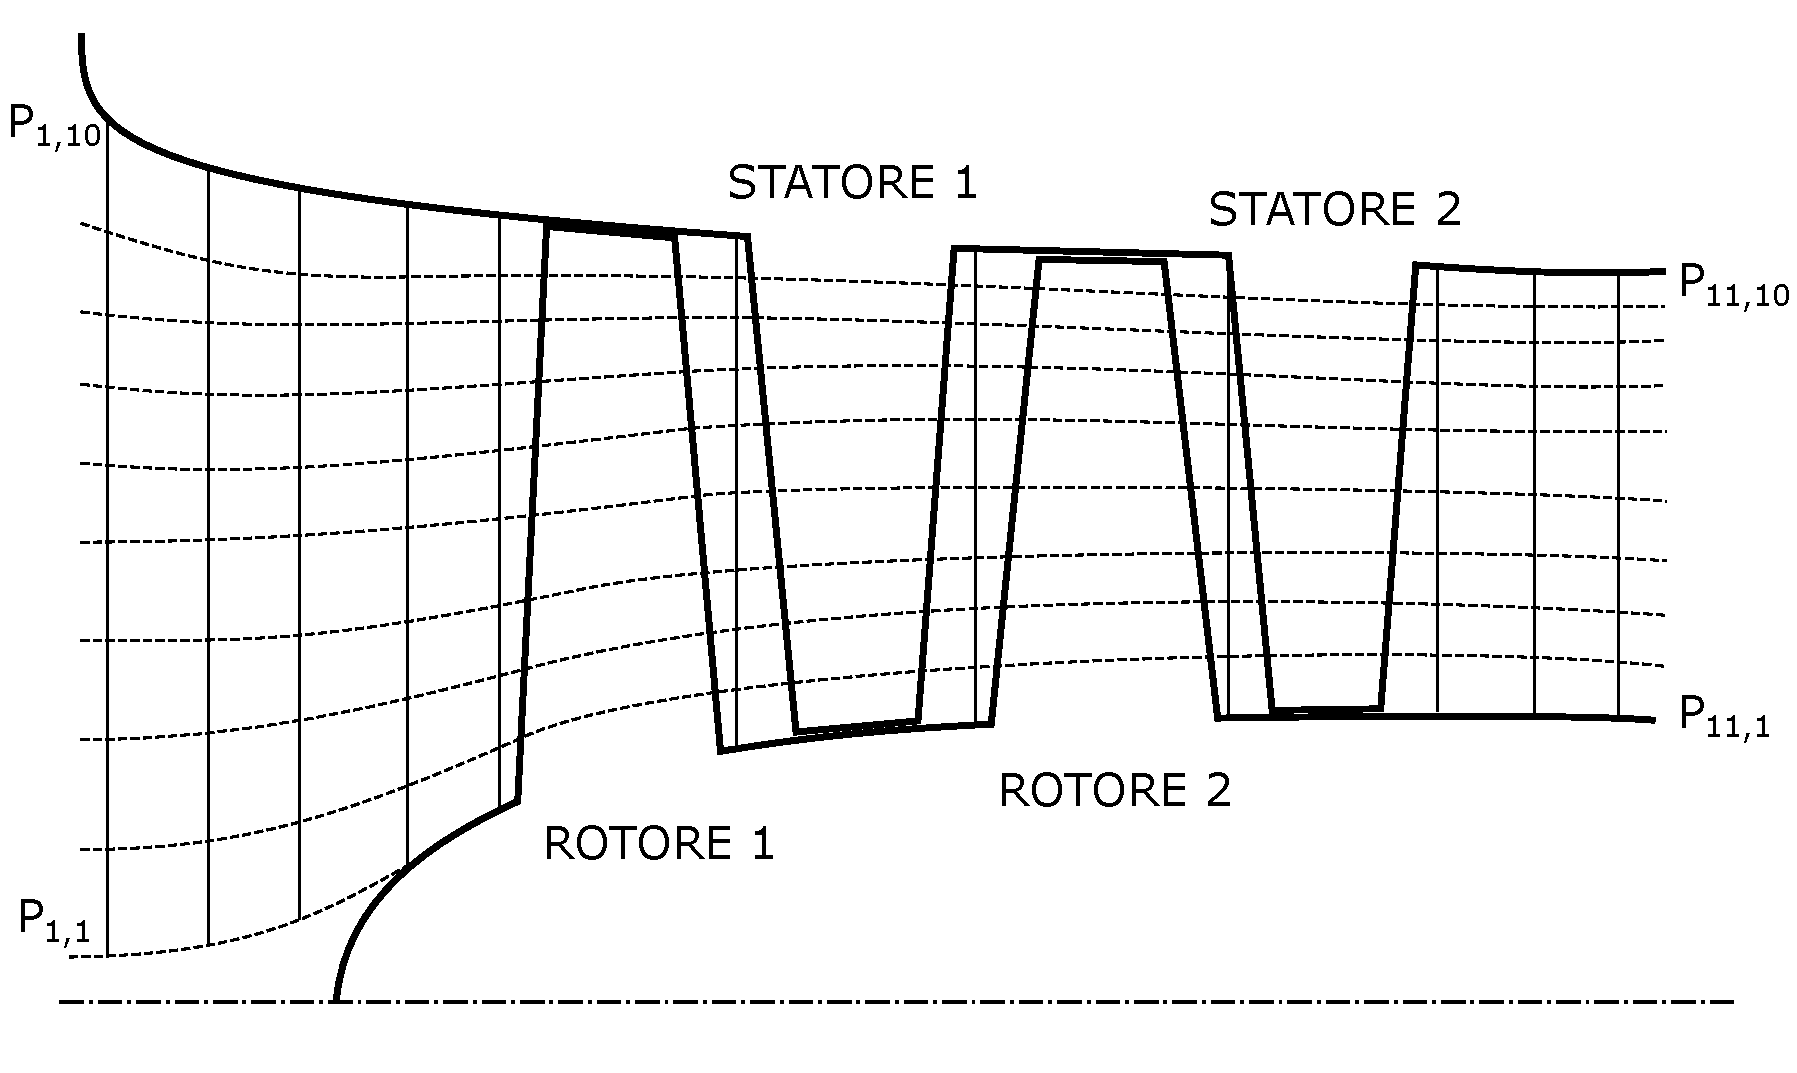
\includegraphics[width=.8\textwidth]{fig/ReticoloComp.pdf}
\caption{Reticolo di calcolo quasi-3D per una sezione di un compressore assiale bistadio}
\label{fig:ReticoloComp1}
\end{figure}
\'E possibile applicare un’analisi di tipo bidimensionale per esempio alla coppia $ROTORE\;2 - STATORE\;2$ in cui lo sviluppo della macchina è quasi perfettamente assiale. Si immagini che le linee di corrente siano parallele all'asse di rotazione e che tutte le sezioni meridiane siano uguali a se stesse, ossia si supponga che le linee di corrente siano assialsimmetriche; nello studio della macchina quindi, si studiano separatamente le due sezioni.\\
Si prenda una linea di corrente e si sezioni la macchina lungo la superficie cilindrica di questa linea. Questa superficie cilindrica andrà a sezionare tutte le pale in corrispondenza dello stesso valore di raggio. Immaginando di prendere la superficie cilindrica, tagliandola lungo una generatrice e stendendola sul piano si trasforma la stella di pale in una schiera piana di pale.\\
Poi lo studio è completato con lo studio del piano meridiano dove si andrà a vedere come cambiano le condizioni del flusso al variare del raggio. Quest'analisi verrà fatta in corrispondenza dei punti contenuti in delle sezioni comprese tra una pala e l’altra.\\
Le linee verticali sono linee che è possibile sempre individuare e che non intersecano le pale; in corrispondenza di queste sezioni ortogonali vengono calcolate le condizioni di equilibrio radiale del flusso. Bisogna sempre supporre di avere l'assialsimmetria. Valutando delle sezioni che intersecano la pala ci sarà un flusso periodico e quindi bisogna considerare delle forze scambiate tra fluido e pala.\\
Quindi i due punti fondamentali dell'analisi bidimensionale sono:
\begin{itemize}
\item studio della schiera di pale;
\item studio dell'equilibrio radiale.
\end{itemize}
Unendo i risultati di questi due studi si ottiene il comportamento della macchina (abbastanza simile a quello reale).
Con l’approccio bidimensionale si trascura il fatto che la linea di corrente non è perfettamente assiale (abbiamo una componente radiale) e si vede che nella sezione studiata il flusso non è perfettamente assialsimmetrico.\\
Tutto quello che sfugge a questa analisi costituisce una serie di strutture di flusso definite flussi secondari che sono funzione del modo in cui sono stati modellizzati i flussi principali.
\section{Nomenclatura}
\begin{figure}[h!]
\centering
\begin{minipage}{.5\textwidth}
  \centering
  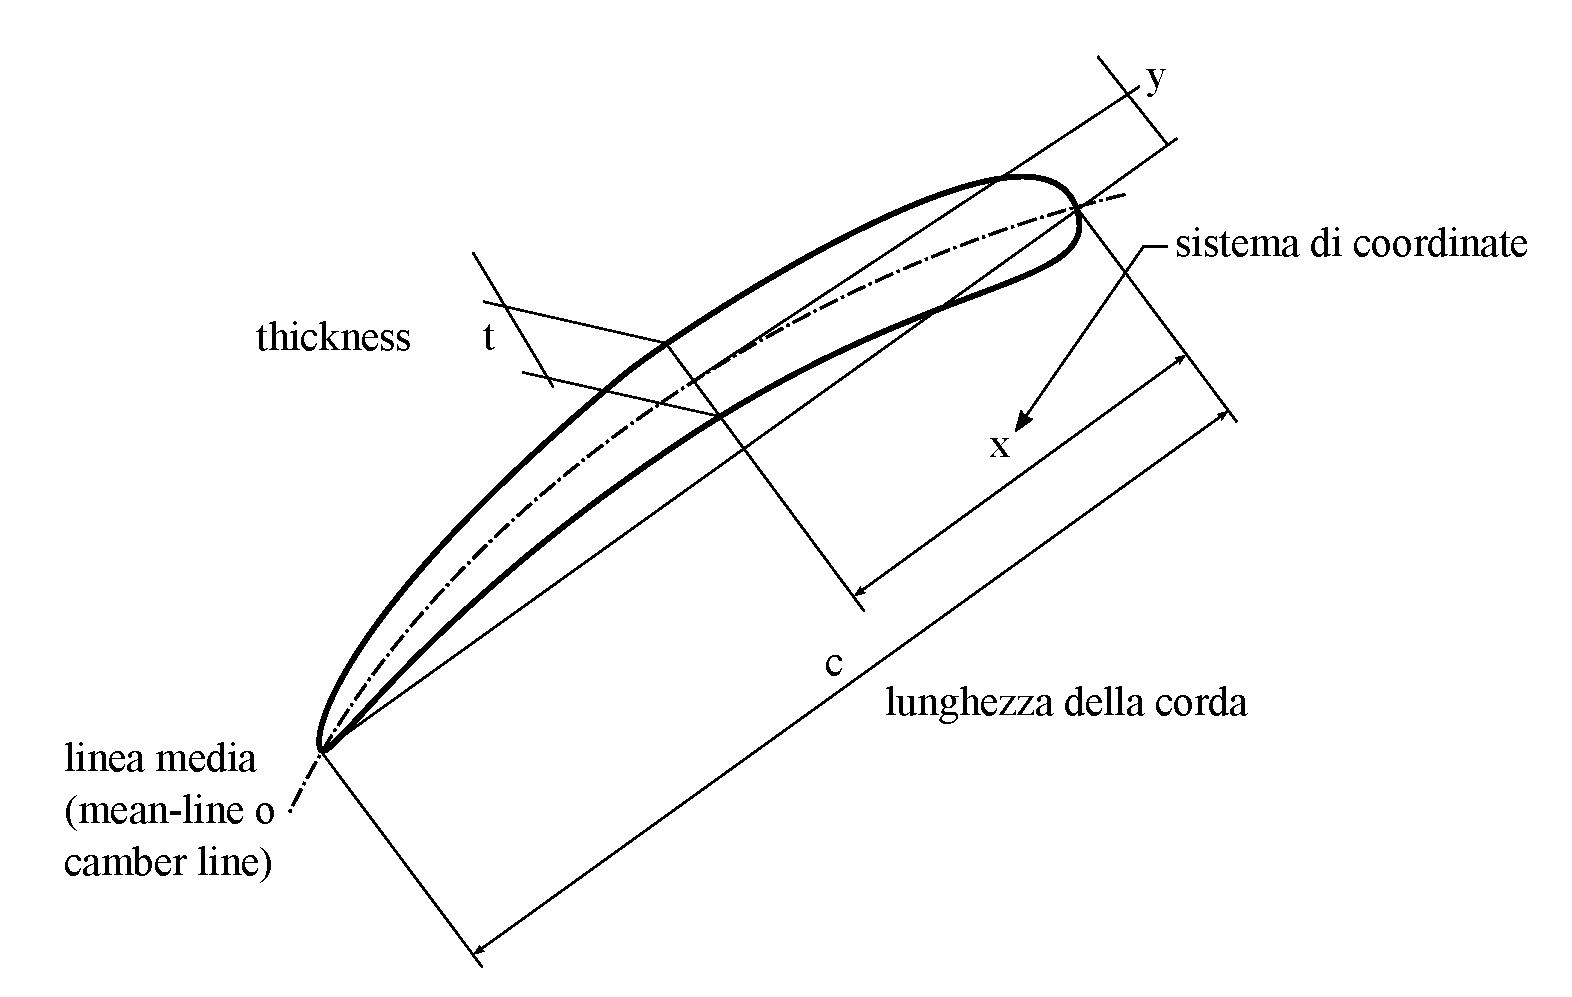
\includegraphics[width=.98\linewidth]{fig/profiloDef.pdf}
  \captionof{figure}{}
  \label{}
\end{minipage}%
\begin{minipage}{.5\textwidth}
  \centering
  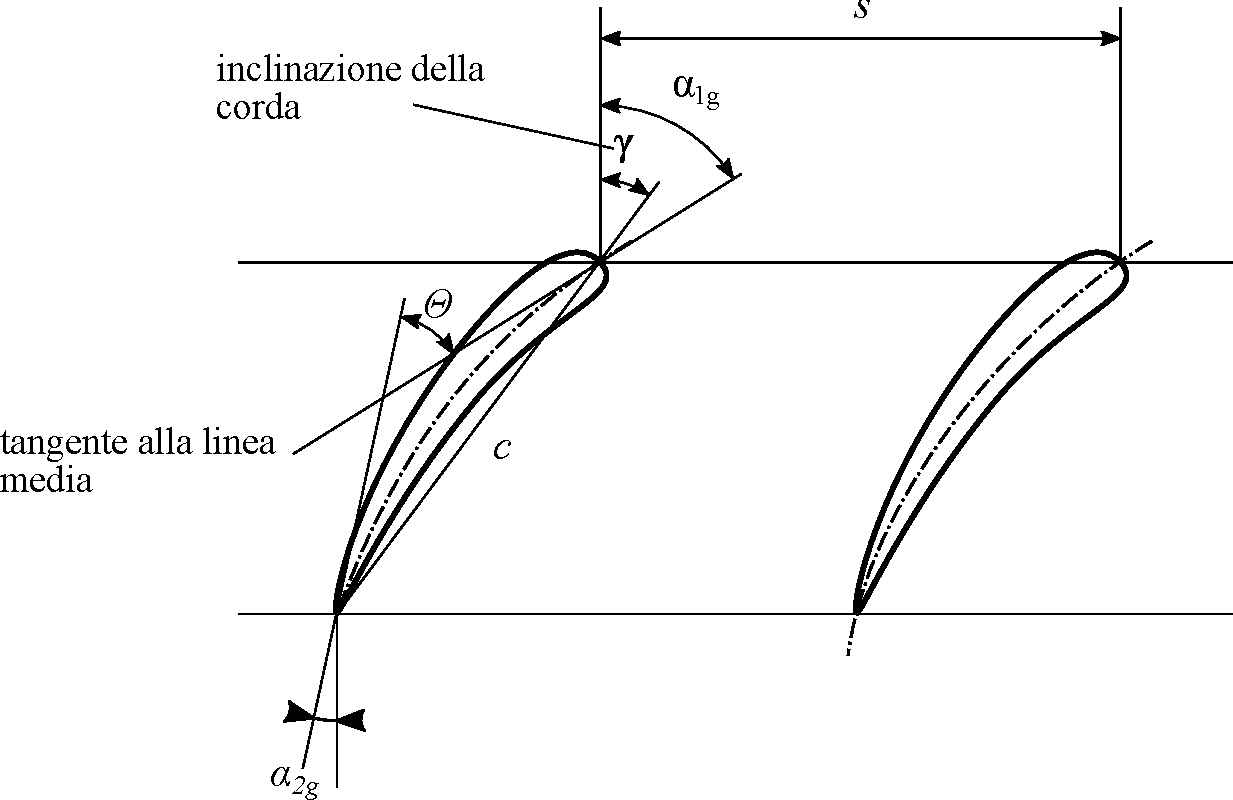
\includegraphics[width=.98\linewidth]{fig/schiera_2.pdf}
  \captionof{figure}{}
  \label{}
\end{minipage}
\end{figure}
Per il profilo isolato si definiscono le seguenti grandezze adimensionali:
\begin{align*}
\cfrac{x}{c} \;\;\;\;\;\; \cfrac{y}{c} \;\;\;\;\;\; \cfrac{t}{c}
\end{align*}
con:\\[1mm]
$t$: spessore massimo del profilo isolato;\\
$c$: lunghezza della corda;\\
$x,y$: coordinate.\\[2mm]
Quanto detto per il profilo isolato varrà anche per i profili in schiera. Come è lecito pensare, nelle applicazioni meccaniche non si limiterà ad una sola pala, ma si considereranno macchine che necessitano di più pale per assolvere al proprio compito. Si definisce quindi la solidità della schiera come
\begin{equation}
\sigma = \cfrac{c}{s}
\end{equation}
con $s$ distanza tra due punti omologhi di due pale successive.
\subsection{Definizioni geometriche}
$\theta$: deflessione geometrica del profilo, differenza tra angolo in ingresso e in uscita (angolo di camber);\\
$\gamma$: angolo di calettamento del profilo della schiera, inclinazione della corda rispetto alla direzione ortogonale);\\
$\alpha_{1g}, \alpha_{2g}$: inclinazioni delle tangenti alla linea media rispetto alla direzione ortogonale\footnote{Il pedice "g" sta per geometrico}.
\begin{align*}
\theta = \alpha_{1g} - \alpha_{2g} = \Delta \alpha_{g}
\end{align*}
\subsection{Definizioni per la corrente fluida}
Immagino poi di investire la mia schiera di pale con una corrente fluida dotata di un certo angolo di incidenza. Si ricavano quindi i seguenti parametri:\\[1mm]
$\alpha_1$: inclinazione del vettore velocità rispetto alla direzione di riferimento ortogonale alla schiera. Una palettatura non riuscirà mai a deviare la corrente tanto quanto è inclinata geometricamente;\\
$\alpha$: angolo di attacco del flusso rispetto la schiera, inclinazione del vettore velocità con riferimento alla corda;\\
$i$: angolo di incidenza, inclinazione del vettore velocità rispetto la tangente alla linea media;\\
$\delta$: angolo di deviazione o deviazione, angolo di deviazione del flusso in uscita rispetto la tangente alla linea media;\\
$\epsilon = \Delta \alpha$: entità della deflessione subita dal flusso tra ingresso e uscita.\\[2mm]
\begin{figure}
\centering
  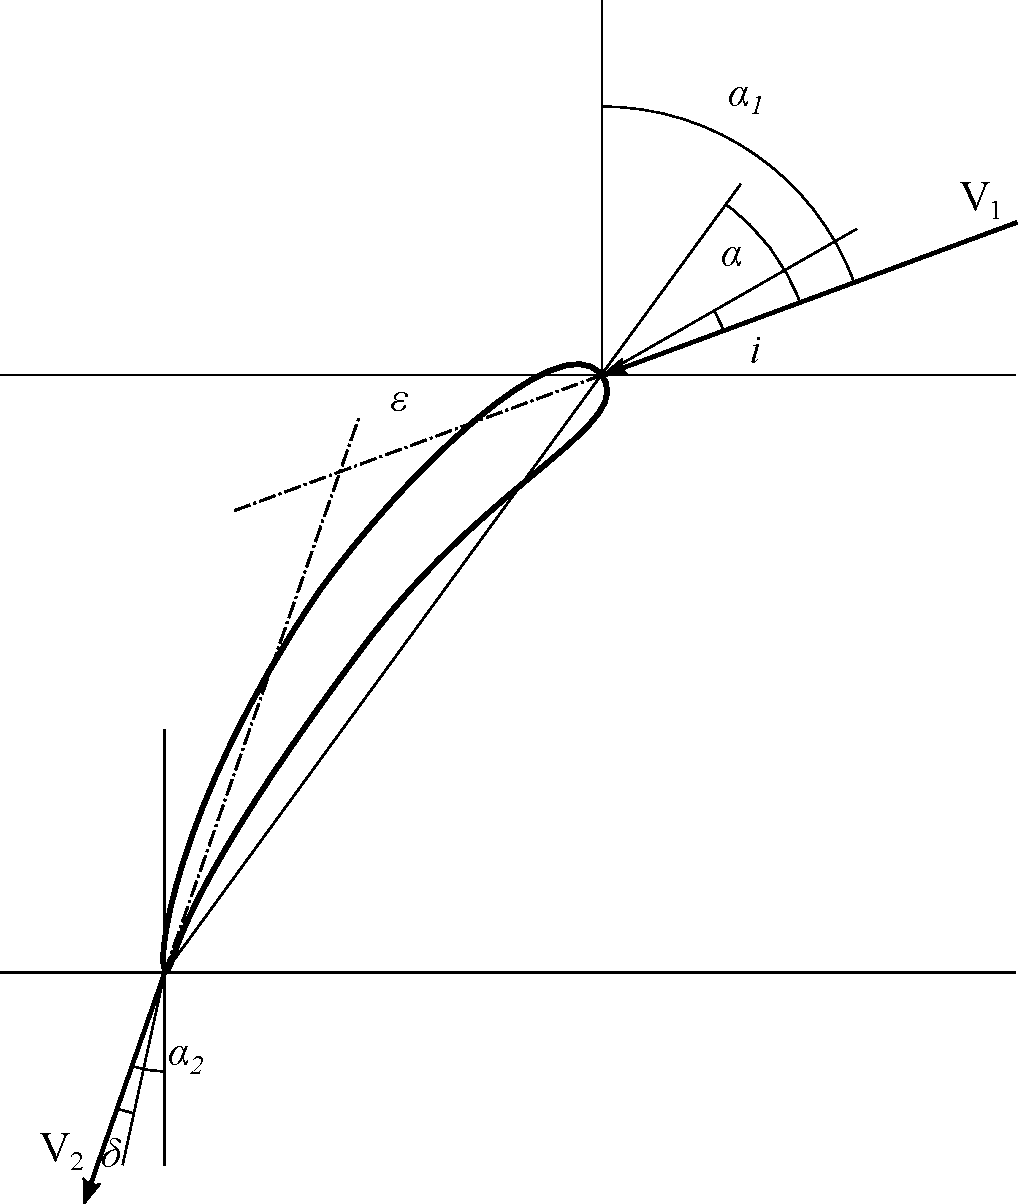
\includegraphics[width=.45\textwidth]{fig/palasing.pdf}
\caption{}
\label{fig:palasing}
\end{figure}
\\Nel caso delle turbine le deviazioni sono più alte rispetto ai compressori visto che rallentare una corrente è sempre molto più facile che accelerarla.\\
Dalle considerazioni geometriche viste prima si può infine scrivere:
\begin{align*}
\varepsilon = \theta + i - \delta
\end{align*}
\subsection{Forze}
Si possono scrivere le forze agenti sulla schiera di pale rispetto al sistema di riferimento assiale - tangenziale per determinare la coppia, ovvero la potenza fornita all'albero nel caso di compressore. La componente assiale sarà la spinta che i cuscinetti dovranno sopportare per il funzionamento e si ripercuote anche sulle perdite di carico.\\
Le stesse forze, poste in un sistema di riferimento diverso (vedi figura \ref{fig:LDref}), sono comunemente note come portanza (Lift) e resistenza (Drag).\\
\begin{align*}
	\begin{cases}
		F_a = f(\Delta v, \Delta p_0)\\
		F_t = f(\Delta v, \Delta p_0)
	\end{cases}
\end{align*}
\begin{align*}
	\begin{cases}
		L = f(F_a,F_t)\\
		D = f(F_a,F_t)
	\end{cases}
\end{align*}
Si consideri ora una schiera palare e un volume di controllo ($ABCD$, di lato minore $s$) che segue la linea media del profilo, figura \ref{fig:schiera1}. Le velocità in ingresso e in uscita vengono scomposte nella direzione assiale e radiale. 
\begin{figure}
\centering
\begin{minipage}{.4\textwidth}
  \centering
  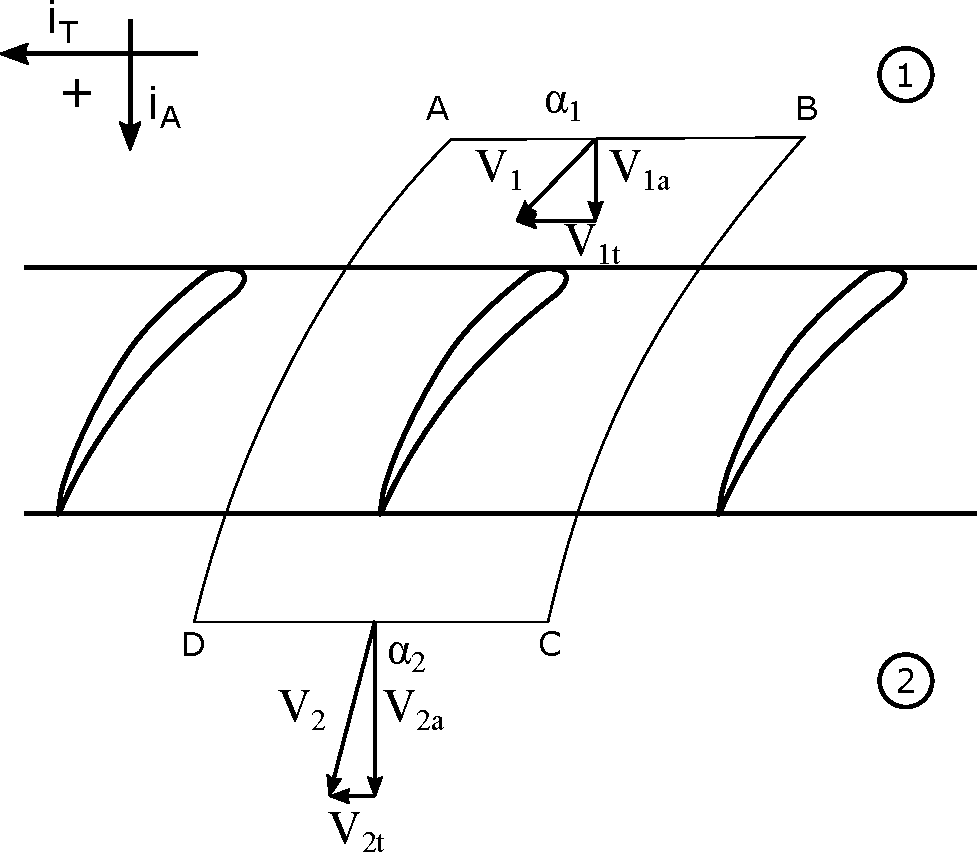
\includegraphics[width=.95\linewidth]{fig/schiera1.pdf}
  \captionof{figure}{}
  \label{fig:schiera1}
\end{minipage}%
\begin{minipage}{.6\textwidth}
  \centering
  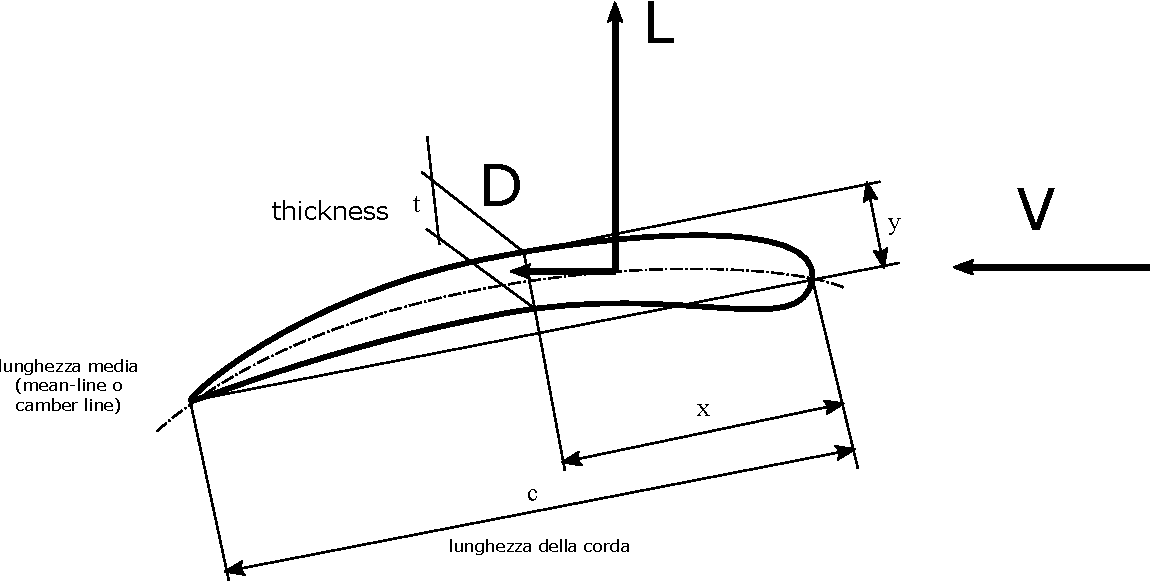
\includegraphics[width=.85\linewidth]{fig/LDref.pdf}
  \captionof{figure}{}
  \label{fig:LDref}
\end{minipage}
\end{figure}
\\Applicando le equazioni di conservazione e scrivendo l'equazione di continuità si ha:
\begin{equation}
s \rho V_{1a} = s \rho V_{2a} \Rightarrow V_{1a} = V_{2a} = V_a
\end{equation}
dove si è ipotizzato $\rho$ costante, in quanto per un compressore assiale i rapporti di compressione per stadio sono modesti (nel caso di una turbina non sarebbe valido). Per quanto riguarda la conservazione della quantità di moto, vale in direzione tangenziale:
\begin{align*}
F_t= \dot{m} \Delta V_t = s \rho	V_a (V_{1t}-V_{2t})
\end{align*}
e in direzione assiale:
\begin{align*}
F_a = s (p_1 - p_2)
\end{align*}
Scrivendo la pressione nelle componenti di pressione statica e dinamica si espande l'espressione per le forze assiali ottenendo:
\begin{align*}
F_a = s \cdot ( p_1 - p_2) &= s \cdot \left( p_{01} - \frac{1}{2} \rho V_1^2 - p_{02} + \frac{1}{2} \rho V_2^2 \right)\\
&= \frac{1}{2} \rho s \left( V_2^2 - V_1^2 \right) + s \left( p_{01} - p_{02} \right)\\
&= \frac{1}{2} \rho s \left( V_{t2}^2 + \cancel{V_a^2} + - V_{t1}^2- \cancel{V_a^2} \right) + s \Delta p_0\\
&=\cfrac{1}{2} \rho s (V_{t2}-V_{t1}) (V_{t2}+V_{t1}) + s \Delta p_0
\end{align*}
con:\\[1mm]
$\Delta p_0$ è la perdita di pressione totale, rappresenta quindi la perdita di carico nel deflusso attraverso la schiera; \\
$(V_{t2}-V_{t1})$ rappresenta il trasferimento di quantità di moto. \\[2mm]
Dividendo il termine $(V_{t2}+V_{t1})$ per $2$ si ottiene l'espressione della velocità tangenziale all'infinito, ossia la velocità media indisturbata:
\begin{align*}
V_{t \infty}=\cfrac{(V_{t2}+V_{t1})}{2}
\end{align*}
Eseguendo ulteriori sostituzioni si trova la relazione fra le forze assiale e tangenziale:
\begin{align*}
F_a = -F_t \cfrac{V_{t \infty}}{V_a} + \Delta p_0 = - F_t \tan \alpha_{\infty} + s \Delta p_0
\end{align*}
con $\alpha_{\infty}$ valore medio tra $\alpha_1$ e $\alpha_2$.\\
Si definisce anche un coefficiente di perdita $y$ come:
\begin{align*}
y = \cfrac{\Delta p_0}{p_{02}-p_2} = \cfrac{\Delta p_0}{\cfrac{1}{2} \rho V_2^2}
\end{align*}
[\textbf{Nota bene}: è stato usato lo stesso simbolo ma non deve essere confuso con il numero di Camber].\\
Nel sistema di riferimento relativo, figura \ref{fig:LDref} e \ref{fig:triang1}, le forze vengono scomposte nella componente di lift, ortogonale alla velocità incidente, e nella componente di drag, parallela alla velocità incidente. La componente di drag è indicativamente sempre un ordine di grandezza inferiore rispetto la componente di lift.
\begin{figure}
\centering
  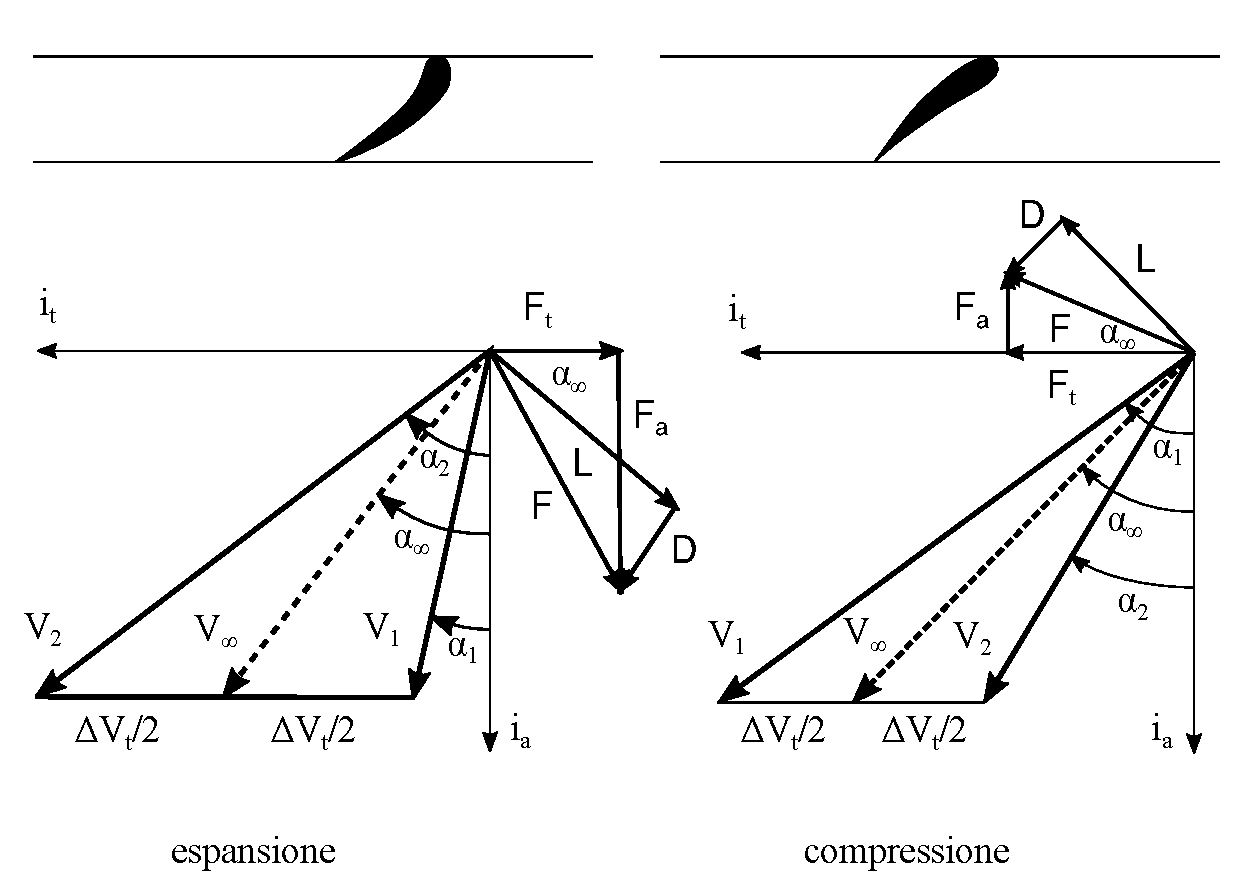
\includegraphics[width=.7\textwidth]{fig/triang1.pdf}
\caption{}
\label{fig:triang1}
\end{figure}
Risulta quindi possibile scrivere le espressioni di lift e drag in funzione delle forze nelle componenti assiale e tangenziale e viceversa:
\begin{equation}
	\begin{cases} 
		L = F_t \cos \alpha_{\infty} -  F_a \sin \alpha_{\infty}\\
		D = F_t \sin \alpha_{\infty} +  F_a \cos \alpha_{\infty}
	\end{cases}
\end{equation}
\begin{equation}
	\begin{cases} 
		F_a = - (L\sin \alpha_{\infty} -  D \cos \alpha_{\infty})\\
		F_t = L \cos \alpha_{\infty} +  D \sin \alpha_{\infty}
	\end{cases}
\end{equation}
\subsection{Adimensionalizzazione delle forze}
\'E possibile a questo punto definire alcuni coefficienti ottenibili come rapporto tra relativa forza ed energia cinetica indisturbata: il coefficiente di drag, $c_D$, quello di lift, $c_L$, e infine quello di forza, $c_F$.\footnote{Ricordando che manca lo "span", cioè sono forze per unità di lunghezza. Questo perché la lunghezza della palettatura è considerata unitaria. Se la pala avesse una profondità sarebbe necessario moltiplicare al denominatore anche per la profondità per ottenere una superficie.}
\begin{align*}
c_L = \cfrac{L}{\cfrac{1}{2} \rho c V_{\infty}^2}
\end{align*}
\begin{align*}
c_D = \cfrac{D}{\cfrac{1}{2} \rho c V_{\infty}^2}
\end{align*}
\begin{align*}
c_F = \cfrac{F_t}{\cfrac{1}{2} \rho c V_{\infty}^2} = \cfrac{s \cancel{\rho} V_a (V_{t1}-V_{t2})}{\cfrac{1}{2} c \cancel{\rho} V_{\infty}^2}
\end{align*}
\begin{figure}
\centering
  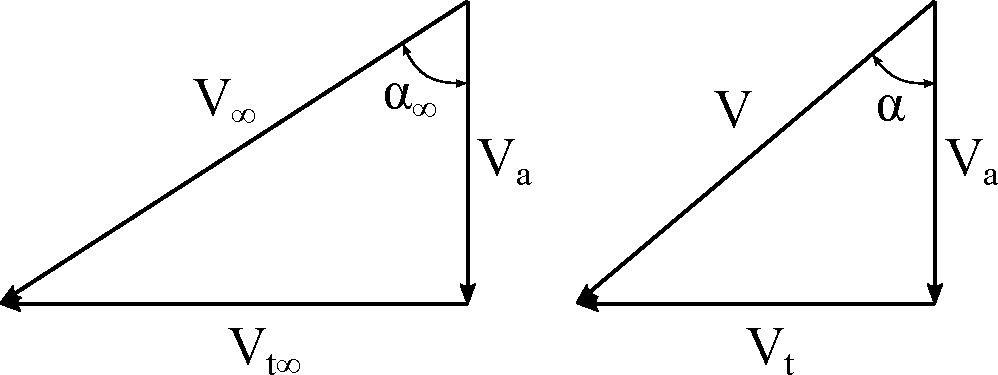
\includegraphics[width=.6\textwidth]{fig/trigrel.pdf}
\caption{}
\label{fig:trigrel}
\end{figure}
Usando le relazioni $V_a = V_{\infty} \cos \alpha_{\infty}$ e $V_{t1,2} = V_a \tan \alpha_{1,2}$ (vedi Figura \ref{fig:trigrel}), si espande ulteriormente la relazione ottenendo:
\begin{equation}
c_F = 2 \bigg(\cfrac{s}{c} \bigg) \cos ^ 2 \alpha_{\infty}(\tan \alpha_1 - \tan \alpha_2)
\end{equation}
Alla luce di ciò, detto $c_P$ il coefficiente di pressione, si può ottenere una sua formulazione in maniera analoga:
\begin{align*}
c_P = \cfrac{F_a}{\cfrac{1}{2} \rho c V_{\infty}^2} = \cfrac{s \Delta p_0 - F_t \tan \alpha_{\infty}}{\cfrac{1}{2} \rho c V_{\infty}^2} = \cfrac{s \Delta p_0}{\cfrac{1}{2} \rho c V_{\infty}^2} - c_F \tan \alpha_{\infty}
\end{align*}
e ricordando la relazione del coefficiente di perdita:
\begin{align*}
y = \cfrac{\Delta p_0}{\cfrac{1}{2} \rho c V_2^2}
\end{align*}
si può scrivere
\begin{align*}
c_P = \bigg(\cfrac{s}{c}\bigg)y \bigg(\cfrac{V_2}{V_{\infty}}\bigg)^2 - c_F \tan \alpha_{\infty}
\end{align*}
e quindi
\begin{equation}
c_P = \bigg(\cfrac{s}{c}\bigg)y \cfrac{\cos^2 \alpha_{\infty}}{\cos^2 \alpha_2} -2\bigg(\cfrac{s}{c}\bigg) \left(\tan \alpha_1 - \tan \alpha_2 \right) \sin \alpha_{\infty} \cdot \cos \alpha_{\infty}
\end{equation} 
Come fatto con le forze, si possono esprimere quindi i coefficienti adimensionali secondo i diversi sistemi di coordinate trovando allora:
\begin{align*}
\begin{cases}
c_L = c_F \cos \alpha_{\infty} - c_P \sin \alpha_{\infty} \\
c_D = c_F \sin \alpha_{\infty} + c_P \cos \alpha_{\infty}
\end{cases}
\end{align*}
Sostituendo $c_F$ e $c_P$ si ottiene:
\begin{equation}
\begin{cases}
c_L = 2 \bigg(\cfrac{s}{c}\bigg) (tan \alpha_1 - \tan \alpha_2) \cos \alpha_{\infty} - c_D \tan \alpha_{\infty} \\
c_D = \bigg(\cfrac{s}{c}\bigg) y \cfrac{cos^3 \alpha_{\infty}}{\cos \alpha_2}
\end{cases}
\end{equation}
Si sono così ottenute tutte le relazioni per passare da coefficienti di portanza e resistenza a coefficienti di forza e pressione. Nel caso di fluido ideale non viscoso il coefficiente di drag è nullo; in questo caso allora il coefficiente di lift dipenderà solo dalla geometria della schiera.
\section{Ipotesi di flusso a potenziale}
Sotto le ipotesi di flusso a potenziale non c'è generazione di forze. Si introduce quindi una singolarità nel flusso, una rotazione, per modellare matematicamente il profilo sfruttando il teorema di Kutta-Jukowsky, il quale fornisce una spiegazione analitica allo svilupparsi della portanza del profilo.\\
Da un punto di vista del potenziale, si somma alla corrente uniforme un vortice libero che causerà una certa circuitazione non nulla attorno ad una qualsiasi linea che racchiude il profilo. Sull'estradosso la velocità sarà maggiore di $V_{\infty}$, pari a $V_{\infty}+u,$ mentre sull'intradosso sarà minore, pari a $V_{\infty}-u$; questa differenza di velocità porta ad una conseguente differenza di pressione che causa lo svilupparsi del lift.\\
Applicando il teorema di Kutta-Jukowsky ad un profilo isolato, è possibile calcolare la circuitazione della velocità lungo una linea $l$ attorno al profilo come:
\begin{align*}
\Gamma = \oint_l \overline{v} \cdot d \overline{l} = 2cu
\end{align*}
e quindi risalire al valore di portanza:
\begin{align*}
L=\rho \Gamma V_\infty
\end{align*}

Si ricorda che l'introduzione del vortice libero serve per simulare l'effetto della presenza dello strato limite, il quale non viene considerato nelle ipotesi di flusso a potenziale con moto uniforme; è appunto questa vorticità che, separandosi dalla superficie del profilo, causa il diverso comportamento delle velocità in uscita tra intradosso ed estradosso.\\
In questo modo, anche senza avere la precisione che si avrebbe in una simulazione fluidodinamica del profilo, è possibile modellare in maniera snella anche una schiera di pale. Basterà prendere un volume di controllo attorno alla singola pala della schiera ed individuare come linea di circuitazione, una che segua esattamente la linea di corrente di attraversamento della schiera (AD e CB in figura \ref{fig:schiera1}).\\
\'E possibile utilizzare questa espressione per definire anche la portanza di una schiera. Il teorema di Kutta-Jukowsky può essere applicato in maniera precisa nel caso in cui non ci siano perdite di carico $\Delta p_0=0$; in questo modo la forza risultante coinciderà con la portanza. Sotto le ipotesi di perdite di carico nulle vale:
\begin{align*}
\begin{cases}
F_a = s \rho V_{\infty t} (V_{2t}-V_{1t})\\
F_t = s \rho V_a (V_{1t}-V_{2t})
\end{cases}
\end{align*}
Si trova il rapporto:
\begin{align*}
	\frac{V_{\infty t}}{V_a}=-\frac{F_a}{F_t} = \tan \alpha_{\infty}
\end{align*}
\begin{figure}
	\centering
	\begin{minipage}{.4\textwidth}
		\centering
		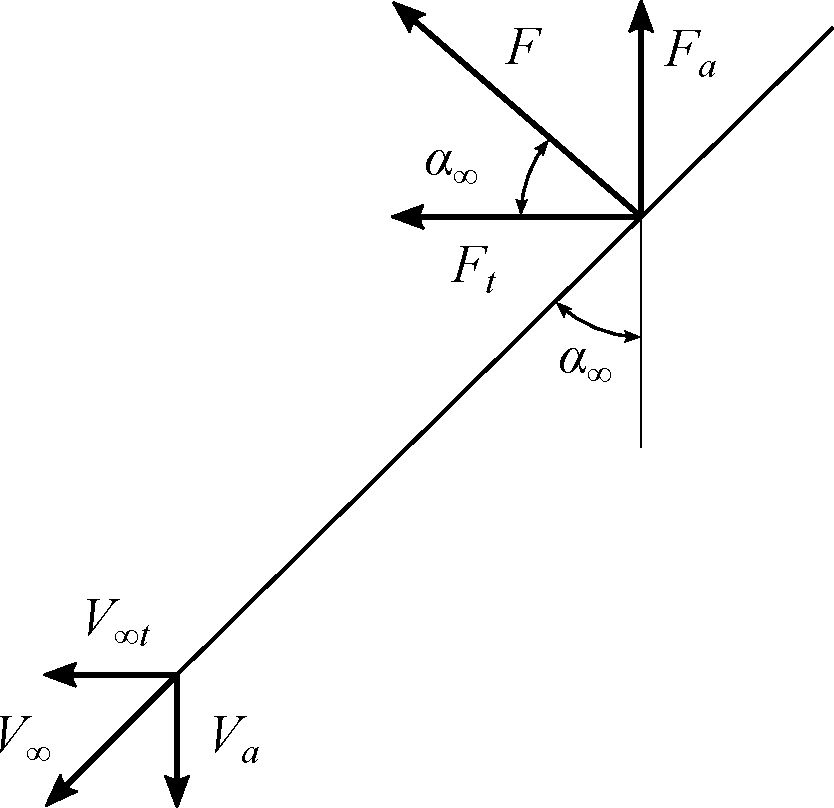
\includegraphics[width=.95\linewidth]{fig/forzaKJ.pdf}
		\captionof{figure}{}
		\label{fig:forzaKJ}
	\end{minipage}
\end{figure}
La forza risultante $F$ è ortogonale a $V_\infty$ e vale:
\begin{align*}
F=\frac{F_t}{\cos \alpha_{\infty}}=\rho \frac{V_a}{\cos \alpha_{\infty}}s(V_{1t}-V_{2t})=\rho V_\infty s (V_{1t}-V_{2t})=L
\end{align*}
Infatti, calcolando la circuitazione lunga una linea s che racchiude un profilo di una schiera di pale e calcolando la portanza con il teorema di Kutta-Jukowsky, viene confermata questa espressione:
\begin{align*}
\Gamma=s(V_{1t}-V_{2t}) \rightarrow L=\rho V_\infty \Gamma
\end{align*}
Questo significa che si trova lo stesso valore di portanza sia nel caso si consideri il profilo nella schiera che lo si consideri isolato utilizzando gli stessi strumenti matematici. Nei due casi cambia però il valore della circuitazione.
\section{Da profilo a schiera} 
\begin{figure}
\centering
\begin{minipage}{.3\textwidth}
  \centering
  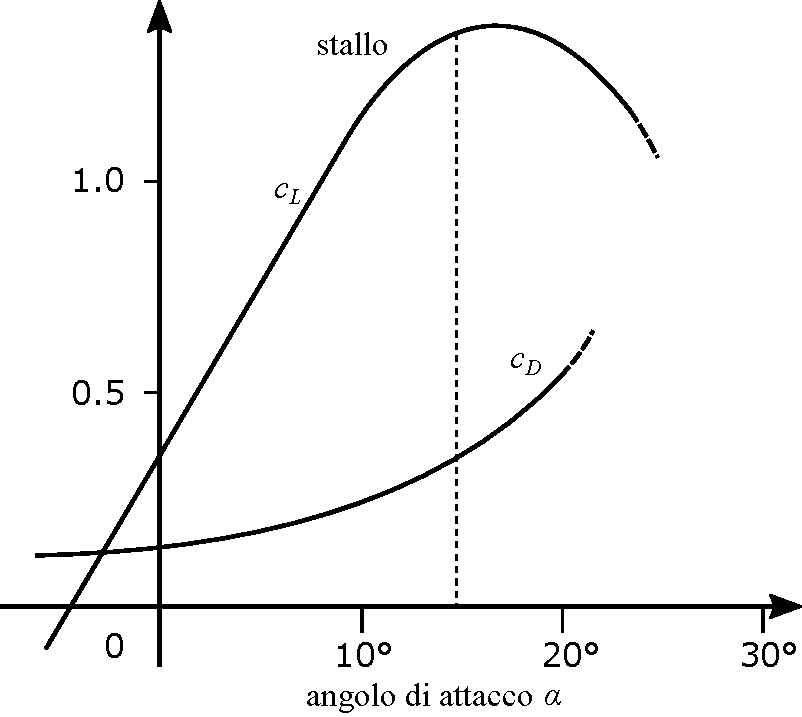
\includegraphics[width=.95\linewidth]{fig/cdcl.pdf}
  \captionof{figure}{}
  \label{fig:cdcl}
\end{minipage}%
\begin{minipage}{.7\textwidth}
  \centering
  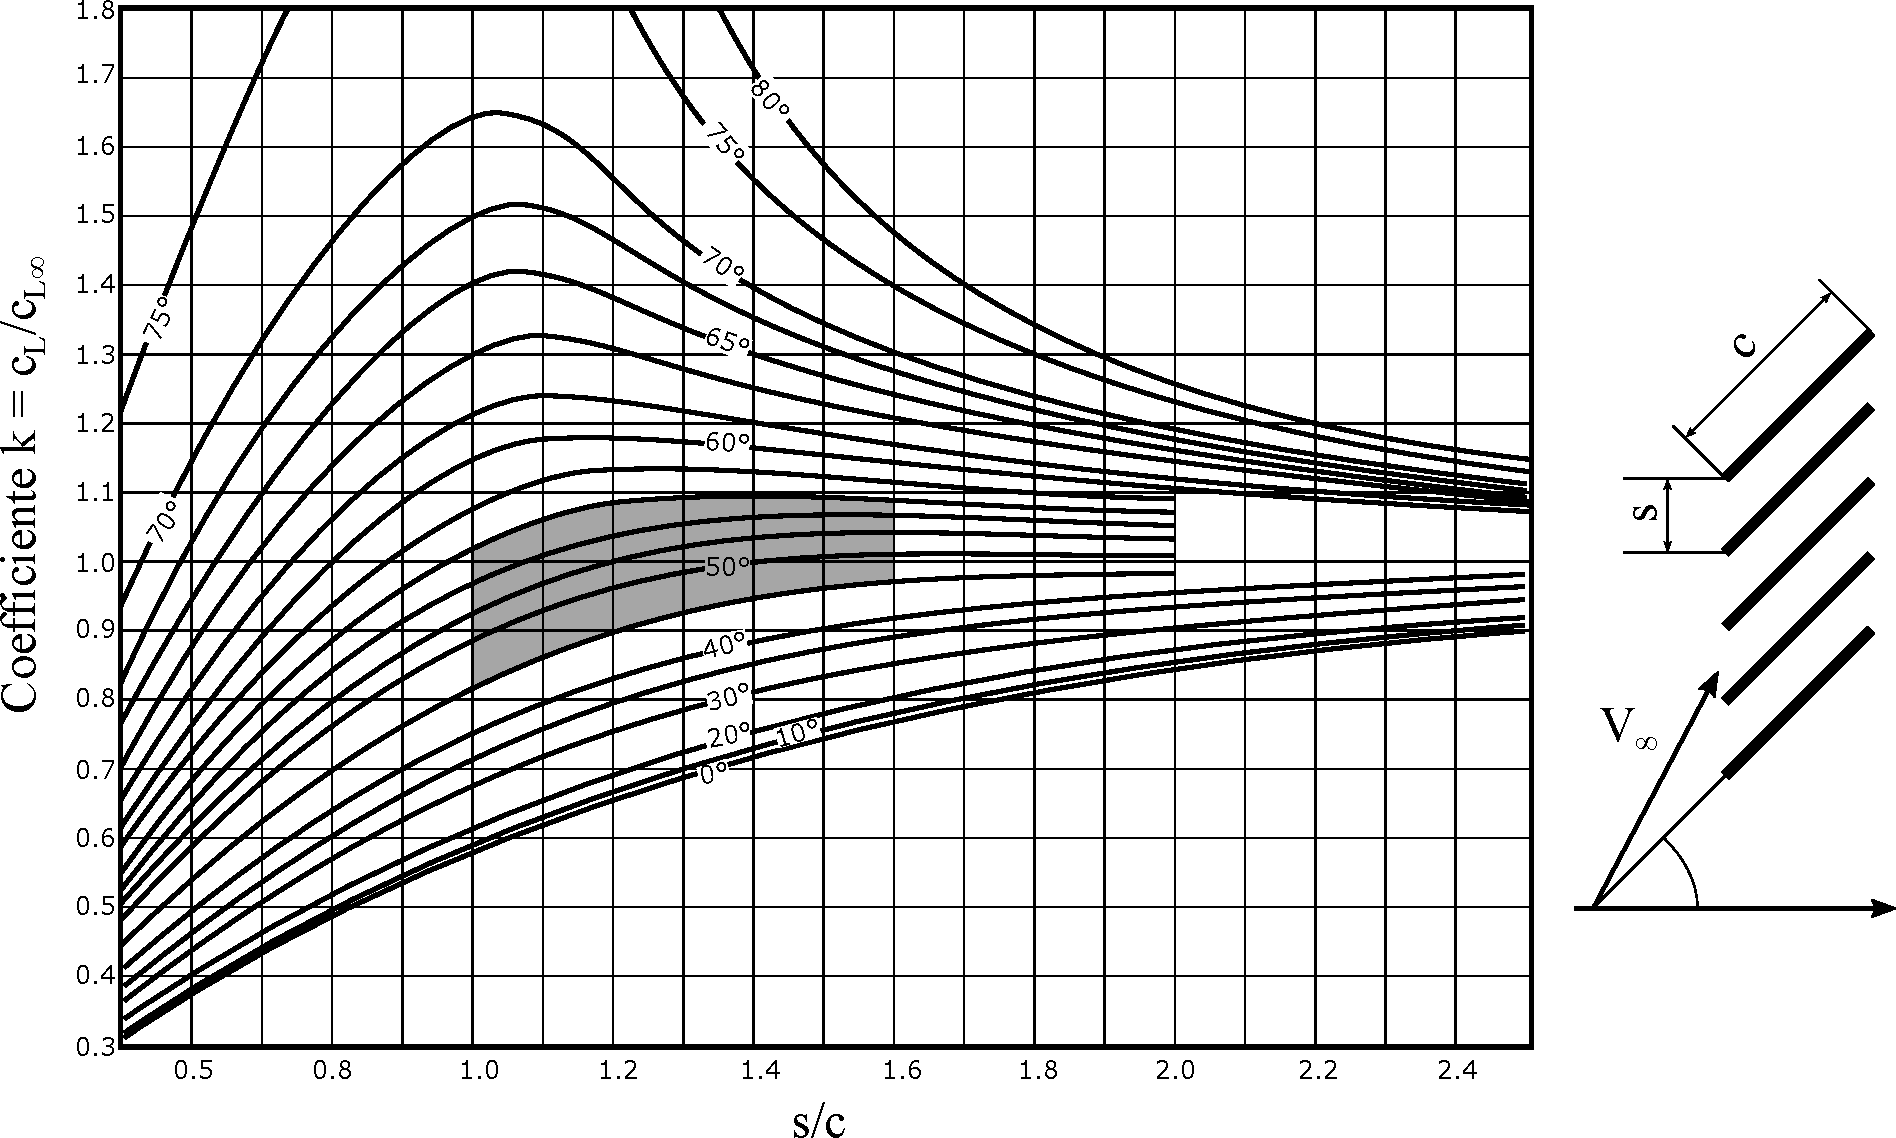
\includegraphics[width=.95\linewidth]{fig/EffSchiera.pdf}
  \captionof{figure}{}
  \label{fig:EffSchiera}
\end{minipage}
\end{figure}
C'è poi la possibilità di correlare per un profilo isolato le relazioni tra angolo di attacco e coefficienti di lift e di drag (Figura \ref{fig:cdcl}). Per quanto riguarda il coefficiente di lift si avrà una parte sostanzialmente lineare mentre il coefficiente di drag è via via crescente. Si arriva ad un punto di stallo in cui c'è una rapida diminuzione del valore di $c_L$ e un rapido aumento di $c_D$; per questo motivo si preferisce lavorare nella zona lineare di variazione di $c_L$. \'E possibile valutare le prestazioni tentando di correlare quello che succede su un profilo e quello che succede su una schiera di assegnata solidità.\\
Statisticamente si diagramma anche cosa succede tra il rapporto tra il coefficiente di lift e coefficiente di lift di profilo isolato, $c_{L \infty}$, e l'inverso della solidità della schiera al variare dell'angolo di attacco (Figura \ref{fig:EffSchiera}). Il range di solidità al quale si fa riferimento varia tra $1$ e $ 1.5 \div 1.6$ non si va oltre $2$. L'angolo di calettamento della schiera è tra i $45^{\circ} \div 52^{\circ}$ come si vede tracciando le linee orizzontali della zona evidenziata nella figura \ref{fig:EffSchiera}. In questo range il rapporto $c_L / c_{L \infty}$ è molto vicino all'unità.\\
In fase di progettazione si usano i dati del profilo isolato e si corregge il coefficiente secondo questi diagrammi. In contesto industriale si simula direttamente una schiera.
\subsection{Ugelli e diffusori}
Le definizioni sono note e stranote (ugelli portano ad un aumento di velocità a fronte di una riduzione di pressione e vengono utilizzati soprattutto nelle turbine, diffusori viceversa e vengono utilizzati soprattutto nei compressori). \'E possibile rappresentare le trasformazioni che si verificano all'interno di ugelli e diffusori sul piano $h-s$ con una trasformazione non isoentropica.
\begin{figure}
\centering
\begin{minipage}{.5\textwidth}
  \centering
  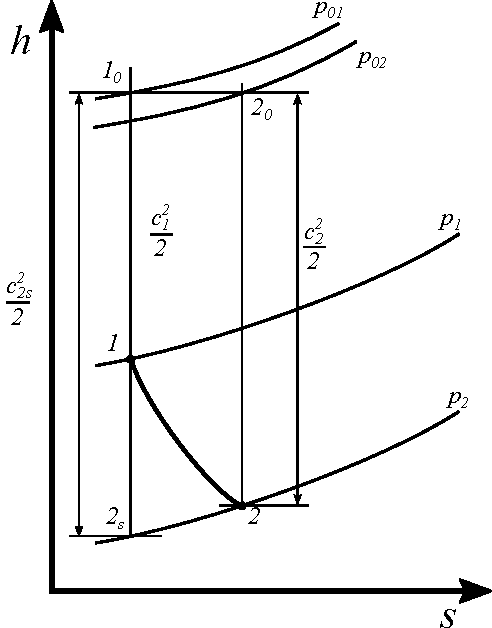
\includegraphics[width=.6\linewidth]{fig/Ugello.pdf}
  \captionof{figure}{Ugello}
  \label{}
\end{minipage}%
\begin{minipage}{.5\textwidth}
  \centering
  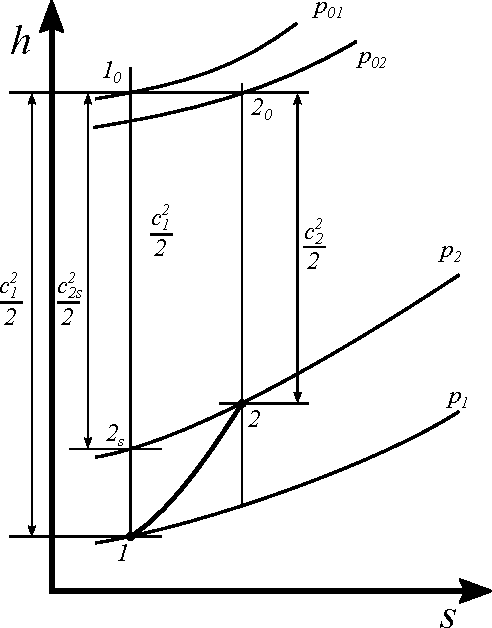
\includegraphics[width=.6\linewidth]{fig/Diffusore.pdf}
  \captionof{figure}{Diffusore}
  \label{}
\end{minipage}
\end{figure}
\\Nel caso di ugelli per $Ma < 0.3$ si può scrivere:
\begin{align*}
\eta_{is} = \cfrac{h_{2s} - h_1}{h_2-h_1} = \cfrac{c_2^2 - c_1^2}{c_{2s}^2 - c_1^2}
\end{align*}
\begin{align*}
\begin{cases}
p_{01} = p_1 + \cfrac{1}{2} \rho c_1^2 \;\;\;\;& \to  \;\;\;\; c_1^2 = \cfrac{2}{\rho} (p_{01} - p_1)\\
p_{02} = p_2 + \cfrac{1}{2} \rho c_{2s}^2 \;\;\;\;& \to  \;\;\;\; c_{2s}^2 = \cfrac{2}{\rho} (p_{01} - p_1)\\
p_{02} = p_2 + \cfrac{1}{2} \rho c_2^2 \;\;\;\;& \to  \;\;\;\; c_2^2 = \cfrac{2}{\rho} (p_{02} - p_2)
\end{cases}
\end{align*}
Sostituendo queste relazioni nell'espressione del rendimento si ottiene:
\begin{align*}
\eta_{is} = \cfrac{p_{02} - p_2 - (p_{01} - p_1)}{\cancel{p_{01}} - p_2 - (\cancel{p_{01}} - p_1)}=\cfrac{p_{02} - p_2 -(p_{01} - p_1)}{p_1-p_2}=1- \cfrac{\Delta p_0}{p_1 - p_2}
\end{align*}
con $\Delta p_0$ che rappresenta la perdita tra ingresso e uscita.\\
Per i diffusori si consideri sempre $Ma<0.3$ e si possono usare le stesse espressioni; si ottiene un rendimento isoentropico come segue:
\begin{align*}
\eta_{is} = \cfrac{p_2 - p_1}{p_2-p_1 + (p_{01}-p_{02})} = \cfrac{c_1^2 - c_{2s}^2}{c_1^2 - c_2^2}
\end{align*}
L'utilizzo di un rendimento isoentropico è meno espressivo nel caso di un diffusore, in quanto ha maggior significato fisico qual è l'entità di $ \Delta p$ recuperabile della parte eccedente la pressione statica in ingresso; quindi:
\begin{align*}
\eta_{is} = \cfrac{p_{01} - p_1 - (p_{01} - p_2)}{p_{01} - p_1-(p_{02} - p_2)} = \cfrac{p_2 - p_1}{p_2 - p_1 + (p_{01} - p_{02})} = \cfrac{1}{1- \cfrac{\Delta p_0}{p_2 - p_1}}
\end{align*}
Definendo il coefficiente di recupero di pressione come:
\begin{align*}
c_p = \cfrac{p_2 - p_1}{p_{01} - p_1}
\end{align*}
si cerca il legame tra coefficiente di recupero di pressione e rendimento isoentropico:
\begin{align*}
\cfrac{1}{\eta_{is}} = \cfrac{p_2 - p_1 + (p_{01} - p_{02})}{p_2 - p_1} = \cfrac{p_{01} - p_1 - (p_{02} - p_2)}{p_2-p_1} = \cfrac{1}{c_P} - \cfrac{p_{02} - p_2}{p_2 - p_1}
\end{align*}
Si può definire un coefficiente di pressione ideale ottenuto ipotizzando di avere un recupero di pressione senza perdite:
\begin{align*}
c_{pi} = \cfrac{p_2 - p_1 + (p_{01} - p_{02})}{p_{01} - p_1}
\end{align*}
che può essere espresso in funzione di $A_1$ e $A_2$, aree di ingresso e uscita del diffusore:
\begin{align*}
c_{pi} = \cfrac{c_1^2 - c_2^2}{c_1^2} = 1 - \left( \cfrac{c_2}{c_1}\right)^2 = 1- \left(\cfrac{A_1}{A_2} \right)^2 =1-\cfrac{1}{A_R^2}
\end{align*}
con $A_R$ aspect ratio (rapporto tra sezione di uscita e sezione di ingresso). A questo punto si ottiene un rapporto:
\begin{align*}
\cfrac{c_P}{c_{pi}} = \cfrac{p_2-p_1}{p_{01}-p_1} \cdot \cfrac{p_{01}-p_1}{(p_1-p_1)+(p_{01}-p_{02})}= \eta_{is}
\end{align*}
Il diffusore funziona bene finché l'aspect ratio è molto piccolo altrimenti si verificano le condizioni per lo stallo a meno di non prevedere un diffusore con una geometria molto allungata. Anche per questo motivo l'angolo $\Theta$ vale pochi gradi soprattutto con diffusori corti, altrimenti ci sarebbe una ricircolazione di flusso sulle pareti e una diminuzione delle prestazioni. 
\begin{figure}
\centering
  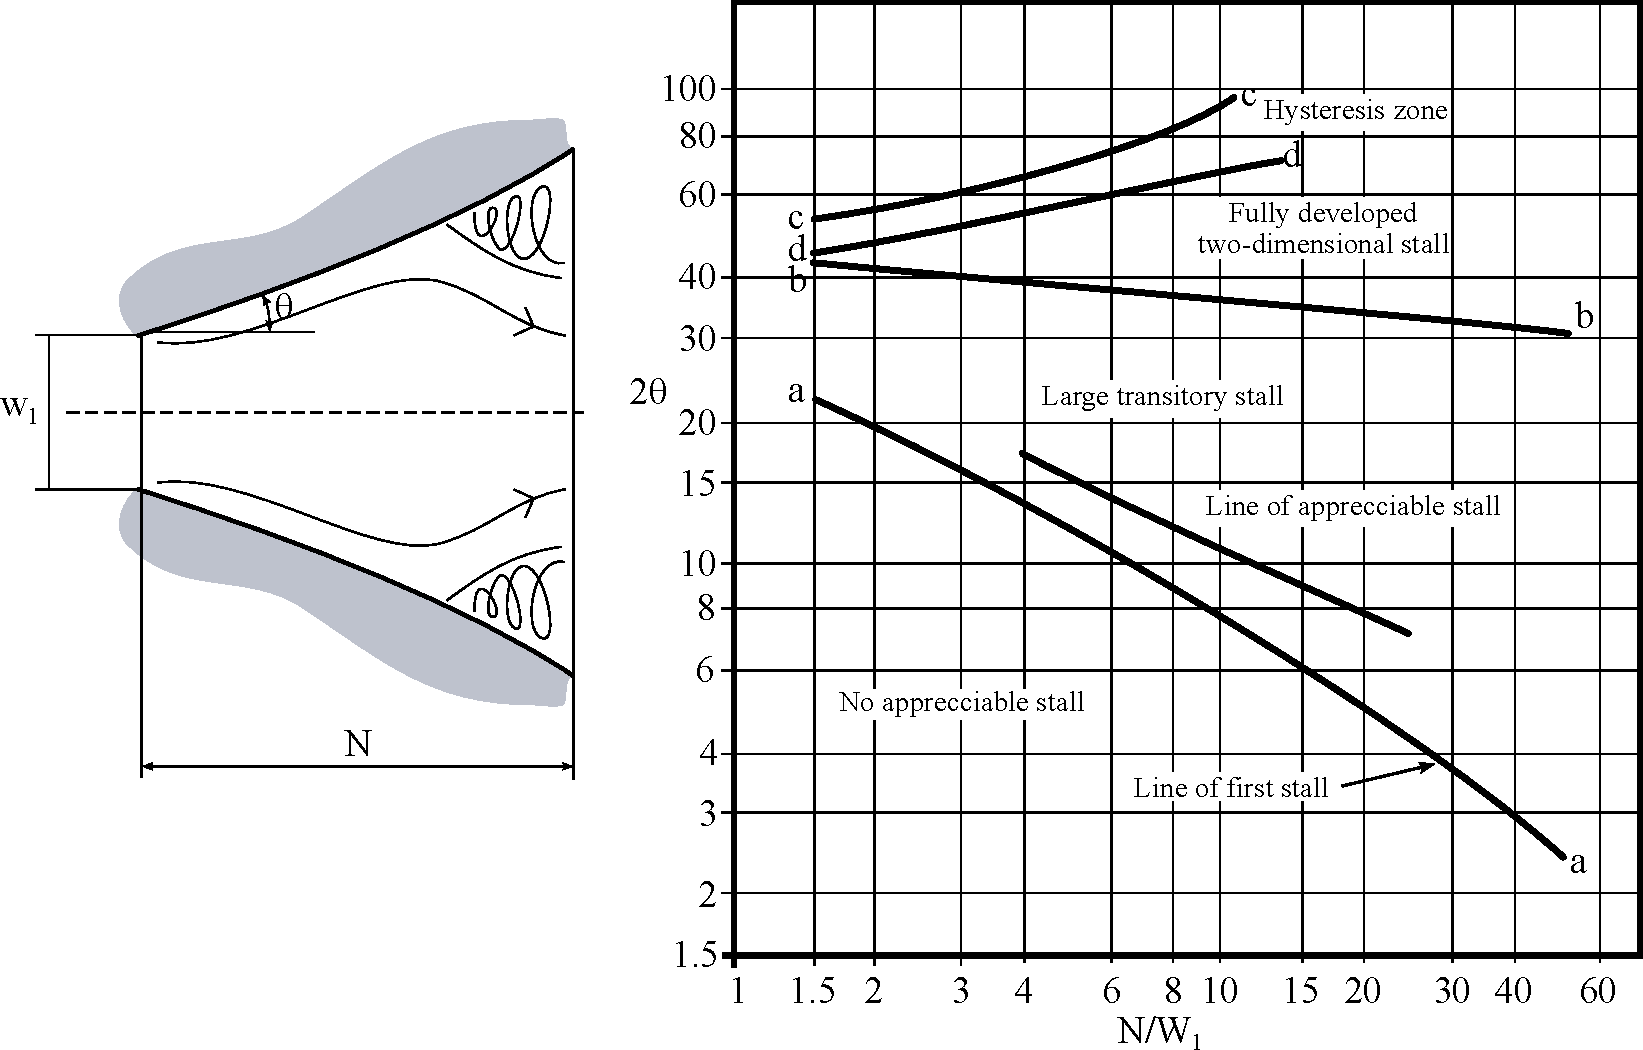
\includegraphics[width=.7\textwidth]{fig/stallo.pdf}
\caption{Zone di stallo}
\label{fig:stallo}
\end{figure}
\begin{figure}
\centering
  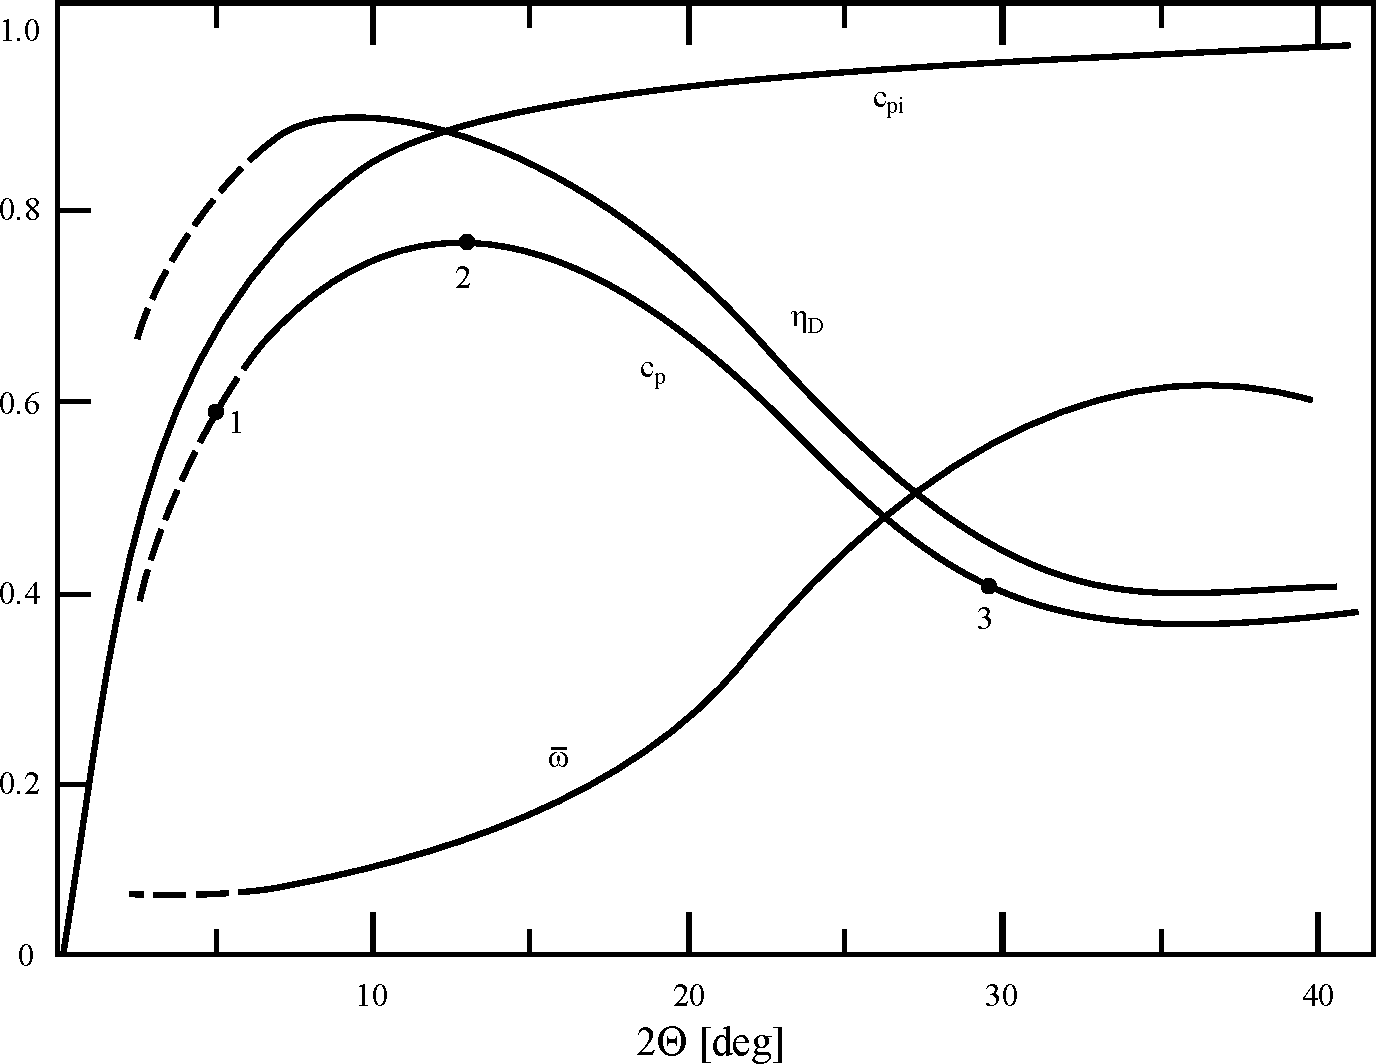
\includegraphics[width=.5\textwidth]{fig/DiffPerf.pdf}
\caption{Tipiche curve di performance per un diffusore bidimensionale con $L/W_1 = 0.8$}
\label{fig:DiffPerf}
\end{figure}
In figura \ref{fig:DiffPerf} sono rappresentate le tipiche curve di un diffusore.
\section{Schiere palari}
Le schiere di pale possono essere:
\begin{itemize}
	\item di espansione, in cui si ha un'accelerazione del flusso e quindi un comportamento simile ad un ugello;
	\item  di compressione in cui si ha una trasformazione della velocità in pressione e quindi un comportamento simile ad un diffusore. 
\end{itemize}
\subsection{Schiere di espansione}
Vista l'analogia con l'ugello, il rendimento isoentropico di queste schiere è espresso come:
\begin{align*}
\eta_{is} = 1- \cfrac{\Delta p_0}{p_1 - p_2}
\end{align*}
Sapendo però che la perdita di pressione tra ingresso e uscita può essere scritta nei termini della forza assiale sviluppata:
\begin{align*}
p_1-p_2 = \cfrac{F_a}{s}
\end{align*}
e la forza assiale può essere scritta come:
\begin{align*}
F_a=  - F_t \tan \alpha_{\infty} + s \Delta p_0
\end{align*}
si può scrivere il rendimento isoentropico come:
\begin{align*}
\eta_{is} = \cfrac{1}{1- \cfrac{\Delta p_0 s}{F_t \tan \alpha_{\infty}}}
\end{align*}
\subsection{Schiere di compressione}
Vista l'analogia con il diffusore, il rendimento isoentropico è espresso come:
\begin{align*}
\eta_{is} = \cfrac{1}{1 + \cfrac{\Delta p_0}{p_2-p_1}}
\end{align*}
Seguendo un percorso simile a quello della schiera di espansione, si possono scrivere le seguenti relazioni:
\begin{align*}
p_2-p_1 = -\cfrac{F_a}{s}
\end{align*}
\begin{align*}
F_a = -F_t \tan \alpha_{\infty} + s \Delta p_0
\end{align*}
\begin{align*}
\eta_{is} = 1- \cfrac{\Delta p_0 s}{F_t \tan \alpha_{\infty}}
\end{align*}
Utilizzando le espressioni viste precedentemente di forza tangenziale, differenza di pressione totale, $V_\infty$ e $V_2$, si risale alla relazione che esprime il secondo termine dell'espressione di $\eta_{is}$:
\begin{align*}
\begin{cases}
F_t = c_F \cfrac{1}{2} \rho c V_{\infty}^2\\
V_{\infty} = \cfrac{V_a}{cos \alpha_{\infty}}\\
\Delta p_0 = y \cfrac{1}{2} \rho V_2^2\\
V_2 = \cfrac{V_a}{cos \alpha_2}
\end{cases}
\;\;\;\; \rightarrow \;\;\;\;
\cfrac{\Delta p_0 s}{F_t \tan \alpha_{\infty}} = \cfrac{y}{c_F \tan \alpha_{\infty}} \cdot \cfrac{cos^2 \alpha_{\infty}}{\delta \cdot cos^2 \alpha_2}
\end{align*}
\\Andando a considerare poi tutte le relazioni tra i coefficienti di forza, di pressione, di lift e di drag è possibile esprimere il rendimento isoentropico in funzione dei parametri di lift e di drag.
\begin{align*}
\begin{cases}
c_P = \left(  \cfrac{s}{c} \right) y \left( \cfrac{V_2}{V_{\infty}}  \right)^2 - c_F \tan \alpha_{\infty}\\
c_L = c_F \cos \alpha_{\infty} - c_P \sin \alpha_{\infty}\\
c_D = c_F \sin \alpha_{\infty} + c_P \cos \alpha_{\infty}
\end{cases}
\;\; \Rightarrow \;\;
\end{align*}
\begin{align*}
\begin{cases}
c_L = 2 \left(  \cfrac{s}{c} \right) (\tan \alpha_1 - \tan \alpha_2) \cos \alpha_{\infty} - c_D \tan \alpha_{\infty}\\
c_D= \left(  \cfrac{s}{c} \right) y \cfrac{\cos^3 \alpha_{\infty}}{\cos \alpha_2}
\end{cases}
\;\; \Rightarrow \;\;
\eta_{is} = 1- \cfrac{2 c_D}{c_L \sin (2 \alpha_{\infty})}
\end{align*}
Per rendere elevato il rendimento della schiera bisogna cercare il massimo del rapporto $c_L/c_D$, che rappresenta quindi l'efficienza del profilo. Esiste un tratto significativo di funzionamento in cui il rapporto $c_L/c_D$ rimane costante e questo corrisponde alle condizioni di funzionamento ottimo.\\
Derivando il rendimento per $\alpha_{\infty}$ si trova il valore dell'angolo che rende massimo il rendimento:
\begin{align*}
\cfrac{\partial \eta_{is}}{\partial \alpha_{\infty}} = 0 \;\;\;\; \cfrac{c_D}{c_L} = cost.
\end{align*}
\begin{align*}
\eta_{is,max} = 1- \cfrac{2 c_D}{c_L}
\end{align*}
Il valore di $\alpha_{\infty}$ ottimale è di $45$ gradi.\\
Secondo la solita convenzione si studiano i triangoli di velocità della schiera in movimento (Figura \ref{fig:SchiereCompr}). I triangoli invece di essere chiusi sul vettore velocità vengono rappresentati partendo dallo stesso punto di origine. 
\begin{figure}
\centering
  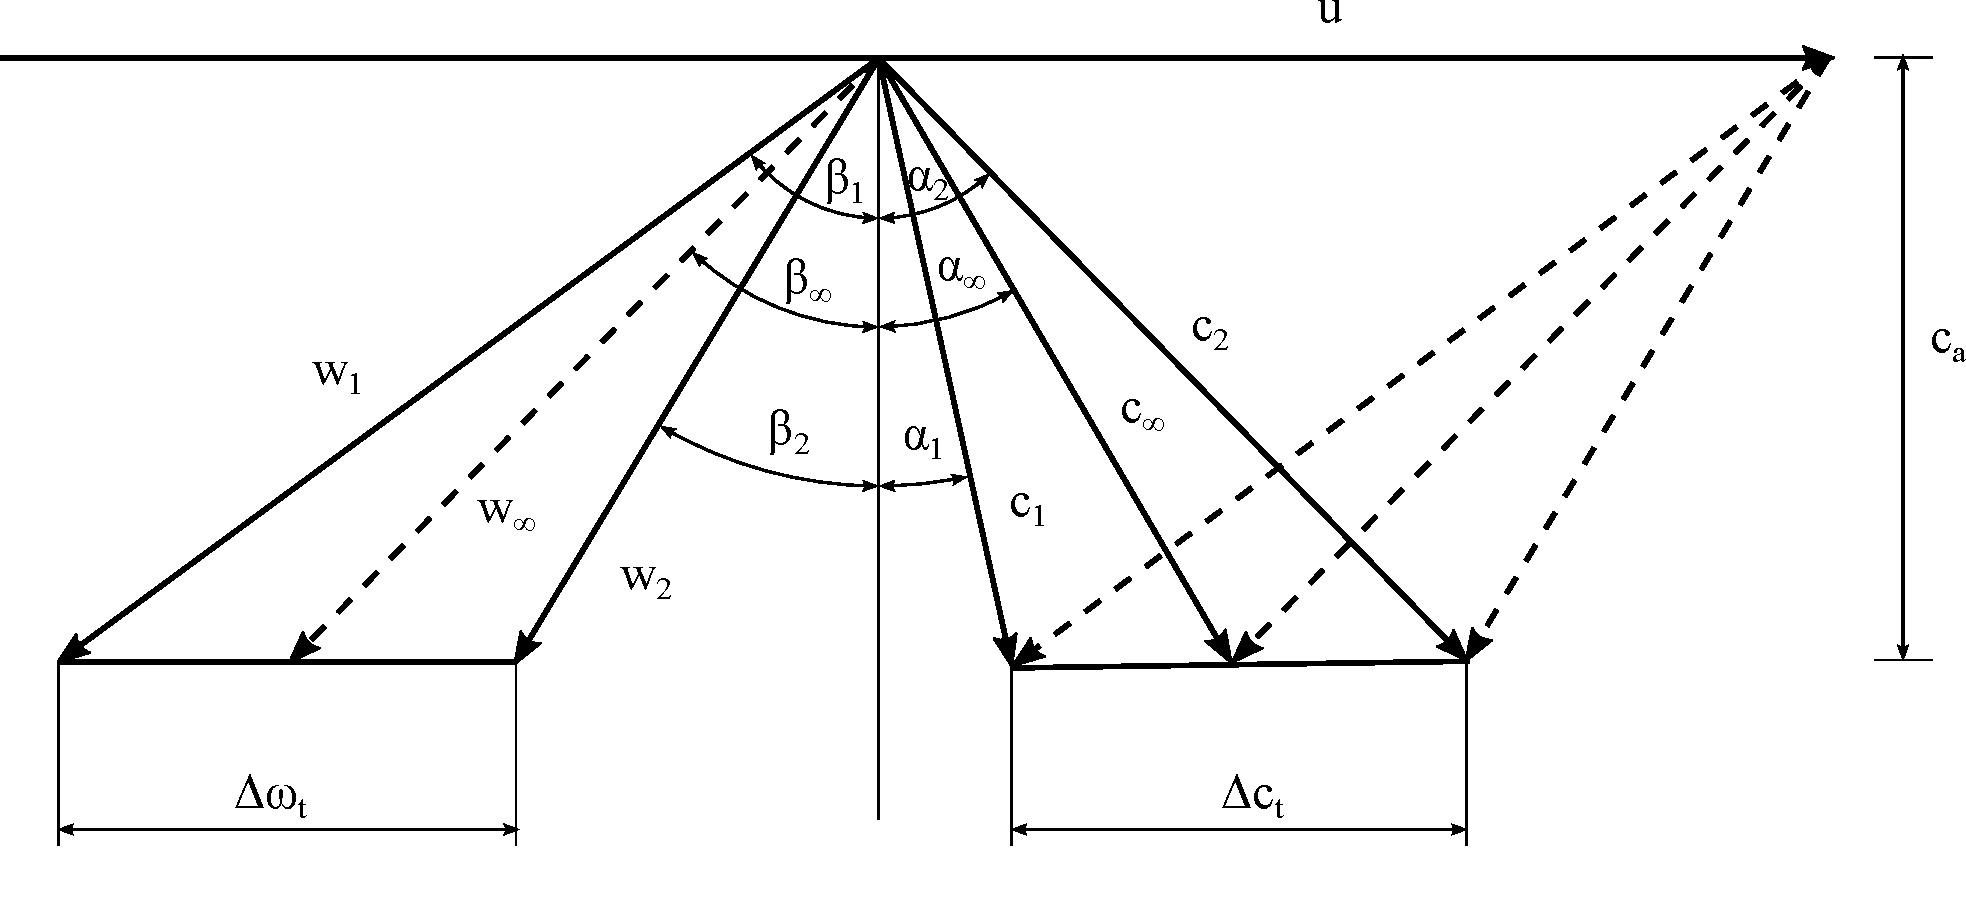
\includegraphics[width=\textwidth]{fig/SchiereCompr.pdf}
\caption{Schiere in movimento (compressore)}
\label{fig:SchiereCompr}
\end{figure}
\\Si può quindi calcolare la forza tangenziale data dalla variazione delle velocità relative tra ingresso e uscita:
\begin{align*}
\Delta c_t = c_{2t} - c_{1t} = \omega_{1t} - \omega_{2t} = |\Delta \omega_t |
\end{align*}
\begin{align*}
F_t = s \rho c_a (\omega_{1t} - \omega_{2t})
\end{align*}
\\Partendo dalle relazioni di potenza, portata in massa e forza tangenziale si definisce il lavoro unitario:
\begin{align*}
\begin{cases}
P=F_t \cdot u\\
\dot{m} = \rho s c_a\\
F_t = c_F \cfrac{1}{2} \rho c \omega_{\infty}^2 = \cfrac{c_F \cfrac{1}{2} \rho c c_a^2}{\cos^2 \beta_{\infty}}
\end{cases} \;\;\;\;
\Rightarrow \;\;\;\;
L_u = \cfrac{F_t \cdot u}{\rho s c_a}
\end{align*}
Sostituendo la relazione della forza tangenziale si ottiene il lavoro unitario in funzione del coefficiente di forza, della solidità della schiera, della velocità assiale e periferica:
\begin{align*}
L_u = \cfrac{c_F \cdot \sigma}{2 \cos^2 \beta_{\infty}} \cdot c_a \cdot u
\end{align*}
\\Con questa espressione si può ora adimensionalizzare il lavoro:
\begin{align*}
\begin{cases}
\lambda = \cfrac{L_u}{\omega ^2 D^2} = \cfrac{L_u}{4 u^2}\\
\varphi = \cfrac{Q}{\omega D^3} \propto \cfrac{c_a}{u}
\end{cases} \;\;\;\;
\Rightarrow \;\;\;\;
\lambda = \cfrac{c_F \delta}{8 \cos^2 \beta_{\infty}} \cdot \cfrac{c_a}{u} = \cfrac{c_F \delta}{8 \cos^2 \beta_{\infty}} \cdot \varphi
\end{align*}
L'ultima espressione rappresenta la curva di funzionamento della macchina in quanto ovviamente il lavoro viene fatto esclusivamente dalle parti rotoriche.\\
Si può quindi scrivere il rendimento isoentropico sia nel caso di compressione che di espansione:
\begin{multicols}{2}
Compressione
\begin{align*}
\eta_{is} = \cfrac{L_u - \cfrac{\Delta p_0}{\rho}}{L_u} = 1- \cfrac{\cfrac{\Delta p_0}{\rho}}{L_u}
\end{align*}
\break
Espansione
\begin{align*}
\eta_{is} = \cfrac{L_u}{L_u + \cfrac{\Delta p_0}{\rho}} = \cfrac{1}{1+\cfrac{\cfrac{\Delta p_0}{\rho}}{L_u}}
\end{align*}
\end{multicols}
e utilizzando le relazioni note:
\begin{align*}
\begin{cases}
\Delta p_0 = y \cfrac{1}{2} \rho \omega_2^2\\
L_u = \cfrac{c_F \delta}{2 \cos^2 \beta_{\infty}} \cdot c_a \cdot u\\
\omega_2 = \cfrac{c_a}{\cos \beta_2}\\
\phi = \cfrac{c_a}{u}
\end{cases}
\end{align*}
si ottengono le espressioni:
\begin{multicols}{2}
Compressione
\begin{align*}
\eta_{is} = 1- \cfrac{y}{c_F} \cdot  \cfrac{cos^2 \beta_{\infty}}{\delta \cos^2 \beta_2} \cdot \phi
\end{align*}
\break
Espansione
\begin{align*}
\eta_{is} = \cfrac{1}{1+\cfrac{y}{c_F} \cdot \cfrac{\cos^2 \beta_{\infty}}{\delta \cos^2 \beta_2} \cdot \phi}
\end{align*}
\end{multicols}
Unendo la parte statorica e parte rotorica, la variazione di pressione che porta al calcolo del rendimento assumerà l'espressione:
\begin{align*}
\Delta p_0 = \Delta p_{0,stat} + \Delta p_{0,rot}
\end{align*}
\section{Equilibrio radiale}
\begin{figure}
\centering
  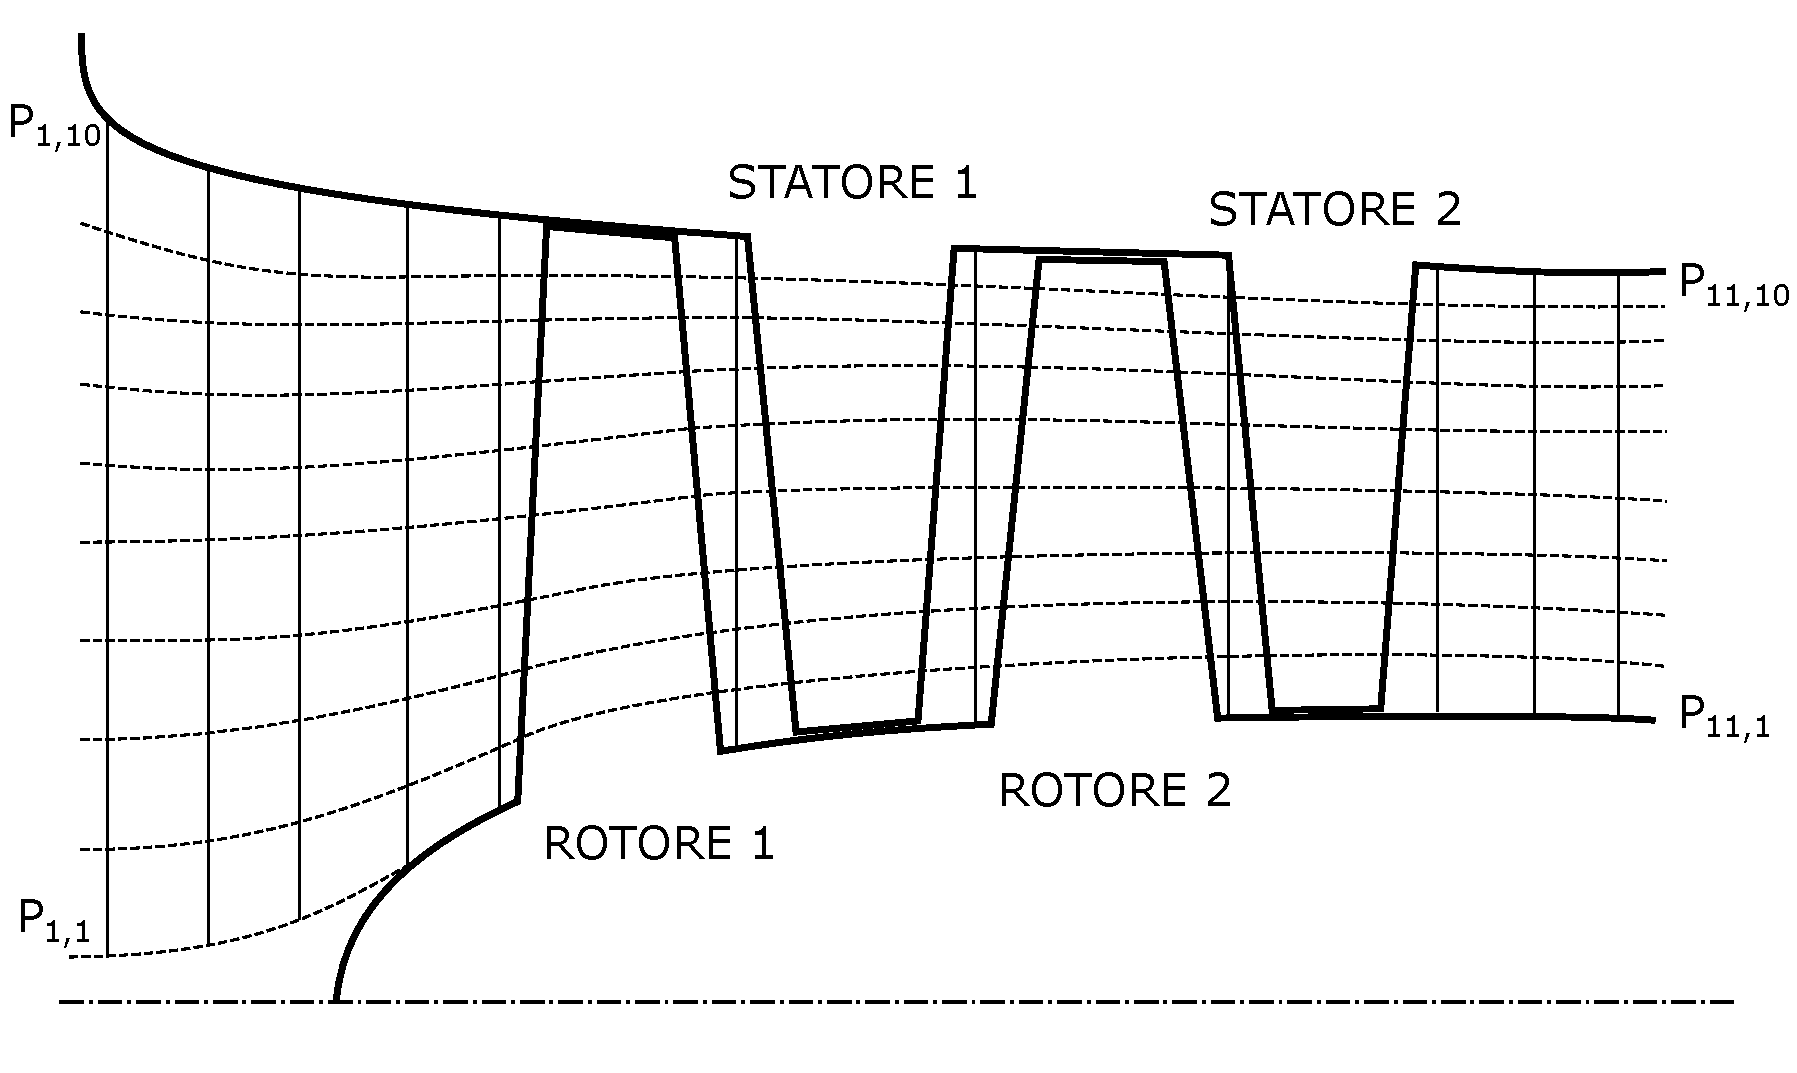
\includegraphics[width=.8\textwidth]{fig/ReticoloComp.pdf}
\caption{Reticolo di calcolo quasi-3D per un compressore assiale bistadio}
\label{fig:ReticoloComp}
\end{figure}
\begin{figure}
\centering
  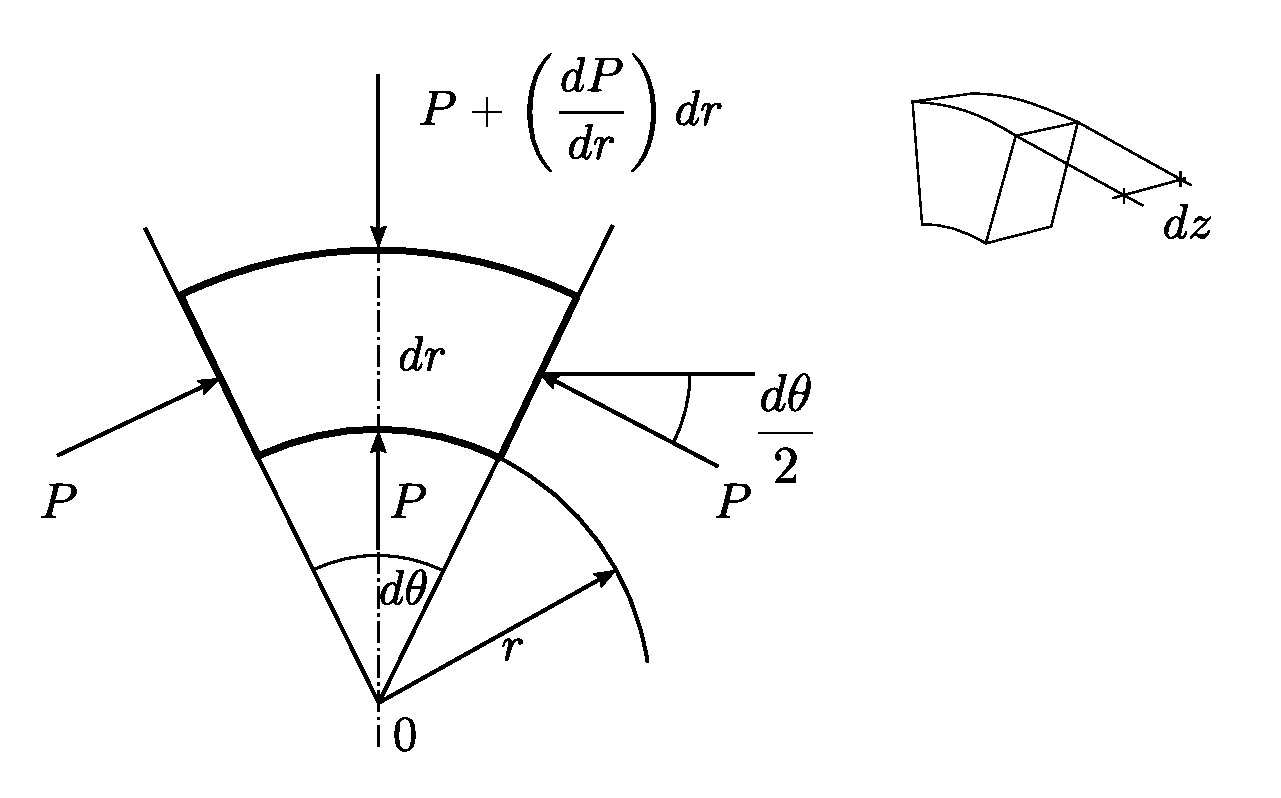
\includegraphics[width=.6\textwidth]{fig/concio.pdf}
\caption{Equilibrio radiale}
\label{fig:concio}
\end{figure}
Con i capitoli precedenti è stato trattato cosa succede nell'attraversamento della schiera in termini macroscopici; per effettuare queste considerazioni bisogna partire dal presupposto che non vi sia un deflusso significativo in direzione radiale assicurandosi quindi che non vi sia trasmissione di forze tra sezioni circolari della macchina.\\
Si consideri ora l'elementino di fluido $dz - d\theta$, figura \ref{fig:concio}, su cui agiscono le forze di pressione. Si calcoli l'equilibrio delle forze:
\begin{align*}
\left( P + \cfrac{dP}{dr} dr \right) (r + dr) d \theta dz - Pr d \theta dz -2P dr dz \sin \frac{d \theta}{2} = r \frac{dP}{dr} dr d \theta dz
\end{align*}
Linearizzando e trascurando i termini del secondo ordine si ottiene un termine che verrà equilibrato dalle forze centrifughe agenti sull'elemento. Affinché il moto non abbia componenti radiali deve quindi accadere:
\begin{equation}
\rho r d \theta dr dz \cdot \frac{V_t^2}{r} = r \frac{dP}{dr} dr d \theta dz \;\;\;\; \Rightarrow \;\;\;\; \cfrac{1}{\rho} \cfrac{dP}{dr} = \frac{V_t^2}{r}
\label{eq:EquilibrioRad}
\end{equation}
\subsection{Termodinamica}
Da un punto di vista termodinamico, si scrive l'entalpia di ristagno (ipotizzando un moto valutato su una superficie cilindrica per cui $V_r = 0$):
\begin{align*}
h_0 = h + \cfrac{V^2}{2} = h + \cfrac{1}{2}(V_t^2 + V_a^2)
\end{align*}
Differenziando lungo il raggio si ottiene:
\begin{equation}
\frac{dh_0}{dr} = \frac{dh}{dr} + V_t \frac{V_t}{dr} + V_a \frac{dV_a}{dr}
\label{eq:EntalpiaDiff}
\end{equation}
Considerando ora il primo principio della termodinamica nella seguente forma:
\begin{equation}
Tds = dh - \cfrac{1}{\rho} dP
\label{eq:PrimoPrinc}
\end{equation}
e unendo le equazioni \ref{eq:EntalpiaDiff} e \ref{eq:PrimoPrinc} risulta:
\begin{align*}
\frac{dh_0}{dr} = T \frac{ds}{dr} + \frac{1}{\rho} \frac{dP}{dr} + V_t \frac{dV_t}{dr} + V_a \frac{dV_a}{dr}
\end{align*}
Considerando poi l'equazione \ref{eq:EquilibrioRad} si ottiene:
\begin{align*}
\frac{dh_0}{dr} = T \frac{ds}{dr} + \frac{V_t^2}{r} + V_t \frac{dV_t}{dr} + V_a \frac{dV_a}{dr}
\end{align*}
In questa espressione non c'è più una pressione ma solo i valori delle velocità, entalpia ed entropia al variare del raggio. A questo punto è possibile scrivere l'equazione complessiva che rappresenta il legame da imporre per avere un flusso bidimensionale:
\begin{align*}
\boxed{ \frac{dh_0}{dr} - T\frac{ds}{dr} = V_a \frac{dV_a}{dr} + \frac{V_t}{r} \frac{d}{dr}(V_t \cdot r)}
\end{align*}
Questa equazione consente di affrontare due problematiche tipiche della progettazione delle macchine:
\begin{enumerate}
\item Problema diretto (o problema di verifica): nota la geometria di una macchina e la distribuzione radiale dell'angolo $\alpha_{\infty}$, determinare la distribuzione radiale di tutte le grandezza del flusso e termodinamiche.
\item Problema inverso (o problema di progetto): assegnata una certa distribuzione di una grandezza termodinamica o fluidodinamica, trovare qual è la geometria della schiera che la realizza.
\end{enumerate}
\subsection{Ipotesi semplificative}
Si può fare un'ulteriore osservazione semplificativa per la fase di progettazione preliminare. Si ipone
\begin{align*}
\begin{cases}
\cfrac{dh_0}{dr} = 0\\
\cfrac{ds}{dr} = 0 
\end{cases}
\end{align*}
ossia che $h_0$ e la dissipazione siano costanti lungo il raggio. In questo modo si ottiene la relazione semplificata:
\begin{equation}
\boxed{ V_a \frac{d V_a}{dr} + \frac{V_t}{r} \frac{d}{dr}(V_t \cdot r) = 0}
\label{eq:EquilibrioRadSemp}
\end{equation}
\section{Condizione di vortice libero}
Queste due osservazioni sono abbastanza realistiche. Dopo aver fatto queste assunzioni sulle distribuzioni delle velocità tangenziali si possono fare delle ulteriori osservazioni sulle velocità assiali.  Ad esempio è possibile costruire la macchina imponendo le condizioni di vortice libero, $V_t \cdot r = cost$.
Questo significa che, considerando un mantello $i$ generico:
\begin{align*}
V_t \cdot r = V_{ti} \cdot r_i
\end{align*}
e unendo l'equazione di vortice libero all'equazione \ref{eq:EquilibrioRadSemp}, si ottiene:
\begin{align*}
V_a=cost
\end{align*}
ossia una velocità assiale costante lungo il raggio.\\
Dal punto di vista dell'entalpia, considerando il rapporto tra una sezione generica e una sezione $i$, sapendo che $h_0 = cost$, si scrive
\begin{align*}
h + \frac{V^2}{2} = h_i + \frac{V_i^2}{2} \Rightarrow h = h_i	+ \frac{V_i^2 - V^2}{2}
\end{align*}
e quindi, considerando che $V^2=V_t^2+V_a^2$:
\begin{equation}
\frac{h}{h_i} = 1 + \frac{1}{2h_i} (V_{ti}^2-V_t^2 + \cancel{V_a^2} -\cancel{V_a^2}) = 1 + \frac{V_{ti}^2}{2h_i} \left( 1- \frac{V_t^2}{V_{ti}^2} \right)
\label{eq:RappEnt}
\end{equation}
Facendo un'ulteriore considerazione:
\begin{align*}
V_t \cdot r = V_{ti} \cdot r_i \Rightarrow \frac{V_t}{V_{ti}} = \frac{r_i}{r}
\end{align*}
riuscendo a scrivere la \ref{eq:RappEnt} come:
\begin{align*}
\frac{h}{h_i} = 1 + \frac{V_{ti}^2}{2h_i} \bigg(1 -  \left( \frac{r_i}{r}\right)^2 \bigg)
\end{align*}
Rimanipolandola ulteriormente si può scriverla nella forma:
\begin{align*}
\boxed{\frac{h}{h_i} = 1 + \frac{\gamma -1}{2} M_{ti}^2 \bigg(1 -  \left( \frac{r_i}{r}\right)^2 \bigg) }
\end{align*}
Si possono ora diagrammare nelle condizioni di vortice libero tutte le espressioni utili a livello termodinamico. In Figura \ref{fig:VorticeLibero} è rappresentata la variazione del rapporto delle pressioni in funzione del rapporto dei raggi al variare del numero di Mach. \'E possibile notare come c'è sempre un valore minimo di raggio oltre il quale non ci si può spingere.
\begin{align*}
\begin{cases}
h = \cfrac{a ^ 2}{\gamma - 1} \\
M_{ti} = \cfrac{V_{ti}}{a_i}\\
\cfrac{h}{h_i} = 1 + \cfrac{\gamma -1}{2} M_{ti}^2 \bigg(1 -  \Big( \cfrac{r_i}{r}\Big)^2 \bigg)\\
\cfrac{p}{p_i} = \left( \cfrac{h}{h_i} \right)^{\frac{\gamma}{\gamma - 1}}
\end{cases}
\end{align*}
\begin{figure}
\centering
  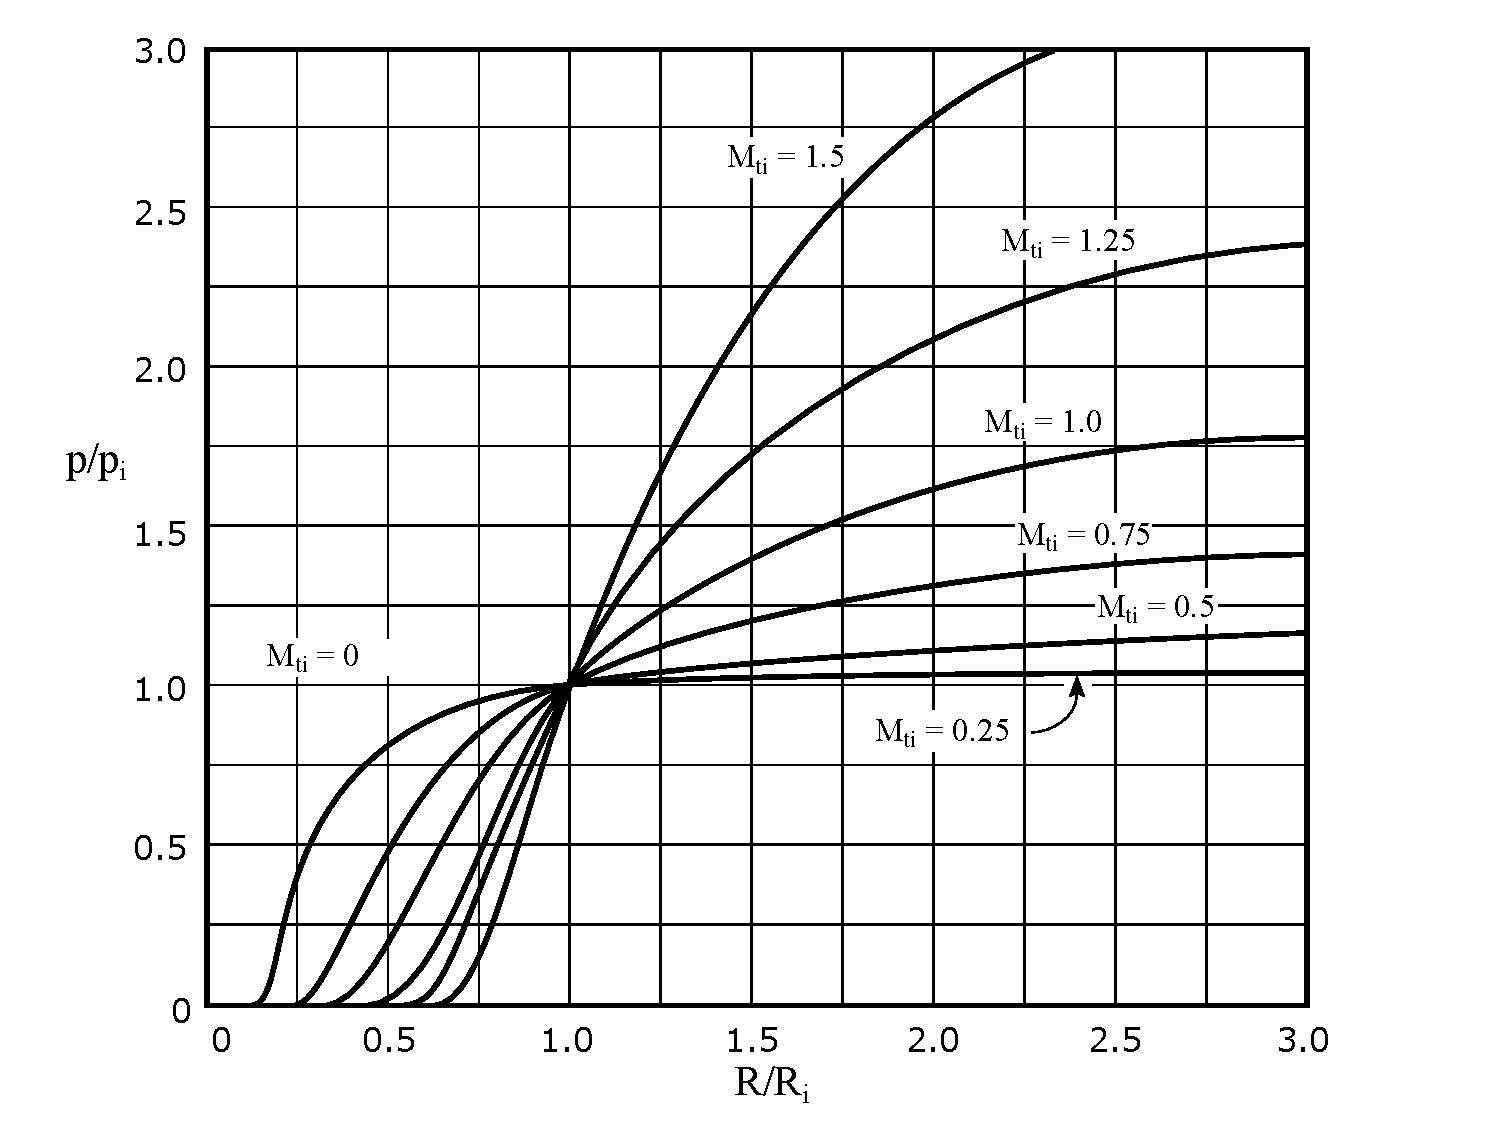
\includegraphics[width=.75\textwidth]{fig/VorticeLibero.pdf}
\caption{Rapporto delle pressioni in funzione del rapporto dei raggi al variare del numero di Mach per un flusso a vortice libero}
\label{fig:VorticeLibero}
\end{figure}
\section{Vortice forzato}
Questo tipo di condizione non si realizza nella realtà nelle fasi di progettazione della macchina o nel suo funzionamento. Tuttavia viene utilizzata per mitigare le problematiche relative al vortice libero introducendo una distribuzione di velocità diversa da quella prevista dal vortice libero.\\
Condizione di vortice forzato:
\begin{equation}
\boxed{\frac{V_t}{r} = cost.}
\label{eq:VortForz}
\end{equation}
Questo significa che il deflusso della macchina si comporta effettivamente come un moto rigido e il rapporto tra velocità tangenziale e raggio si mantiene costante.\\
Si ricordano le equazioni di partenza, ovvero quella di equilibrio radiale e le ipotesi semplificative:
\begin{equation}
\begin{cases}
\cfrac{dh_0}{dr} - T\cfrac{ds}{dr} = V_a \cfrac{dV_a}{dr} + \cfrac{V_t}{r} \cfrac{d}{dr}(V_t \cdot r)\\
\cfrac{dh_0}{dr} - T\cfrac{ds}{dr} = 0
\end{cases}
\label{eq:vorticeForzato}
\end{equation}
Allora considerando la generica sezione $i$:
\begin{align*}
\frac{V_t}{r} = \frac{V_{ti}}{r_i} \;\;\;\; \Rightarrow \;\;\;\; V_t = V_{ti} \frac{r}{r_i}
\end{align*}
Introducendo questa relazione e sostituendola a $V_{t}$ in \ref{eq:vorticeForzato}, si ottiene:
\begin{align*}
\frac{d}{dr}\bigg( \frac{V_a^2}{2} \bigg) + \frac{V_{ti}}{r_i} \frac{d}{dr} \bigg(\frac{V_{ti}}{r_i} r^2 \bigg) = 0
\end{align*}
Si tratta di un'equazione differenziale del primo ordine, risolvibile analiticamente.
\begin{equation}
\frac{d}{dr} \bigg( \frac{V_a^2}{2} \bigg) = -2 \bigg( \frac{V_{ti}}{r_i} \bigg) ^2 \cdot r
\;\;\;\; \Rightarrow \;\;\;\; 
\bigg( \frac{V_a^2}{2} \bigg) = -2 V_{ti}^2 \bigg(\frac{r}{r_i} \bigg)^2 +C
\label{eq:SolCost}
\end{equation}
Bisogna determinare la costante $C$. Nella sezione i-esima la velocità assiale e raggio avranno rispettivamente valori $V_{ai}$ e $r_i$, quindi:
\begin{align*}
\begin{cases}
V_a=V_{ai}\\
r=r_i
\end{cases}
\;\;\;\; \Rightarrow \;\;\;\;
C = \frac{V_{ai}^2}{2} + V_{ti}^2
\end{align*}
Sapendo che:
\begin{align*}
\frac{V_{ti}}{V_{ai}} = \tan \alpha_i
\end{align*}
si può scrivere la \ref{eq:SolCost} nella forma completa:
\begin{equation}
\boxed{ \bigg( \frac{V_a}{V_{ai}} \bigg)^2 = 1- 2 \tan^2 \alpha_i \bigg[ \bigg( \frac{r}{r_i} \bigg)^2 -1 \bigg] }
\label{eq:RappVol}
\end{equation}
Si prosegue e si determina anche l'andamento dell'entalpia in funzione del raggio. Si ricorda l'espressione per l'entalpia totale:
\begin{align*}
h = h_i + \frac{V_i^2 - V^2}{2}
\end{align*}
A questo punto si calcola il rapporto tra l'entalpia di riferimento e l'entalpia in una generica sezione $i$:
\begin{align*}
\frac{h}{h_i} = 1+ \frac{1}{2 h_i} (V_{ti}^2 - V_t^2 + V_{ai}^2 -V_a^2)
\end{align*}
Raccogliendo i termini $V_{ti}$ e $V_{ai}$ si ottiene:
\begin{align*}
\frac{h}{h_i} = 1+ \frac{V_{ti}^2}{2 h_i} \bigg[ 1- \bigg( \frac{V_t}{V_{ti}} \bigg)^2 \bigg] + \frac{V_{ai}^2}{2 h_i} \bigg[ 1- \bigg( \frac{V_a}{V_{ai}} \bigg)^2 \bigg]
\end{align*}
Si possono fare delle ulteriori considerazioni ricordando la \ref{eq:RappVol} e le seguenti espressioni:
\begin{align*}
\begin{cases}
\cfrac{V_t}{V_{ti}} = \cfrac{r}{r_i}\\
\cfrac{V_{ti}}{V_{ai}} = \tan \alpha_i
\end{cases}
\end{align*}
Con alcuni passaggi algebrici si perviene a:
\begin{equation}
\boxed{ \frac{h}{h_i} = 1+ \frac{V_{ti}^2}{2h_i} \bigg[ \bigg( \frac{r}{r_i} \bigg)^2 -1 \bigg] }
\label{eq:rappEntalpie}
\end{equation}
Questo significa che a seconda dell'angolo di incidenza della palettatura, la distribuzione delle velocità assiali non è più uniforme lungo il raggio; si vede chiaramente questo comportamento nel diagramma in Figura \ref{fig:TurboFan}.
\begin{figure}
\centering
  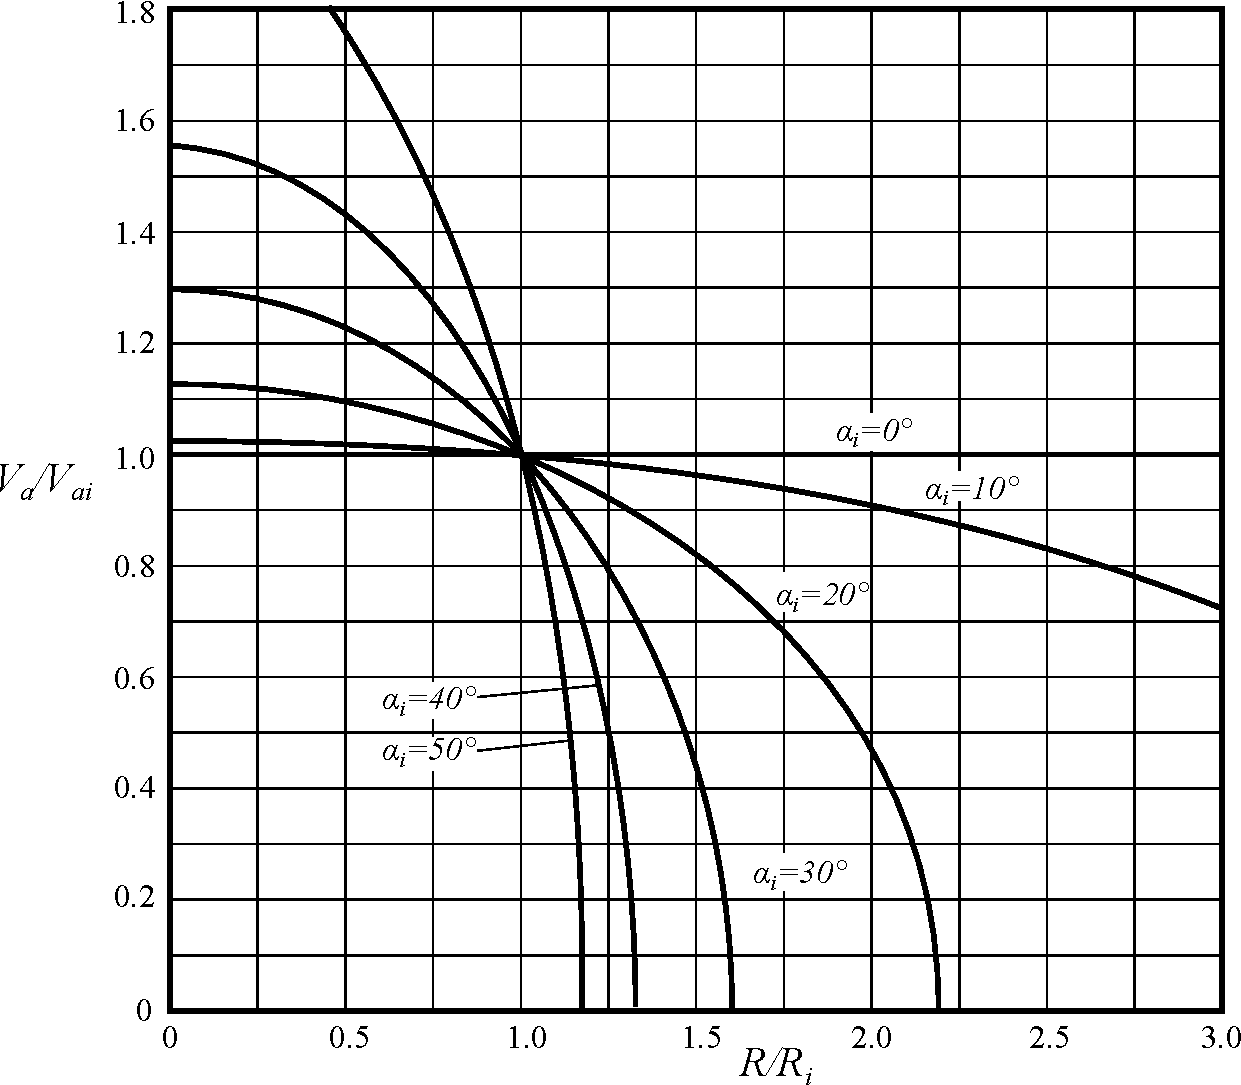
\includegraphics[width=.8\textwidth]{fig/VortForz.pdf}
\caption{Velocità assiale in funzione del raggio per un flusso a vortice forzato}
\label{fig:TurboFan}
\end{figure}
\begin{figure}
\centering
  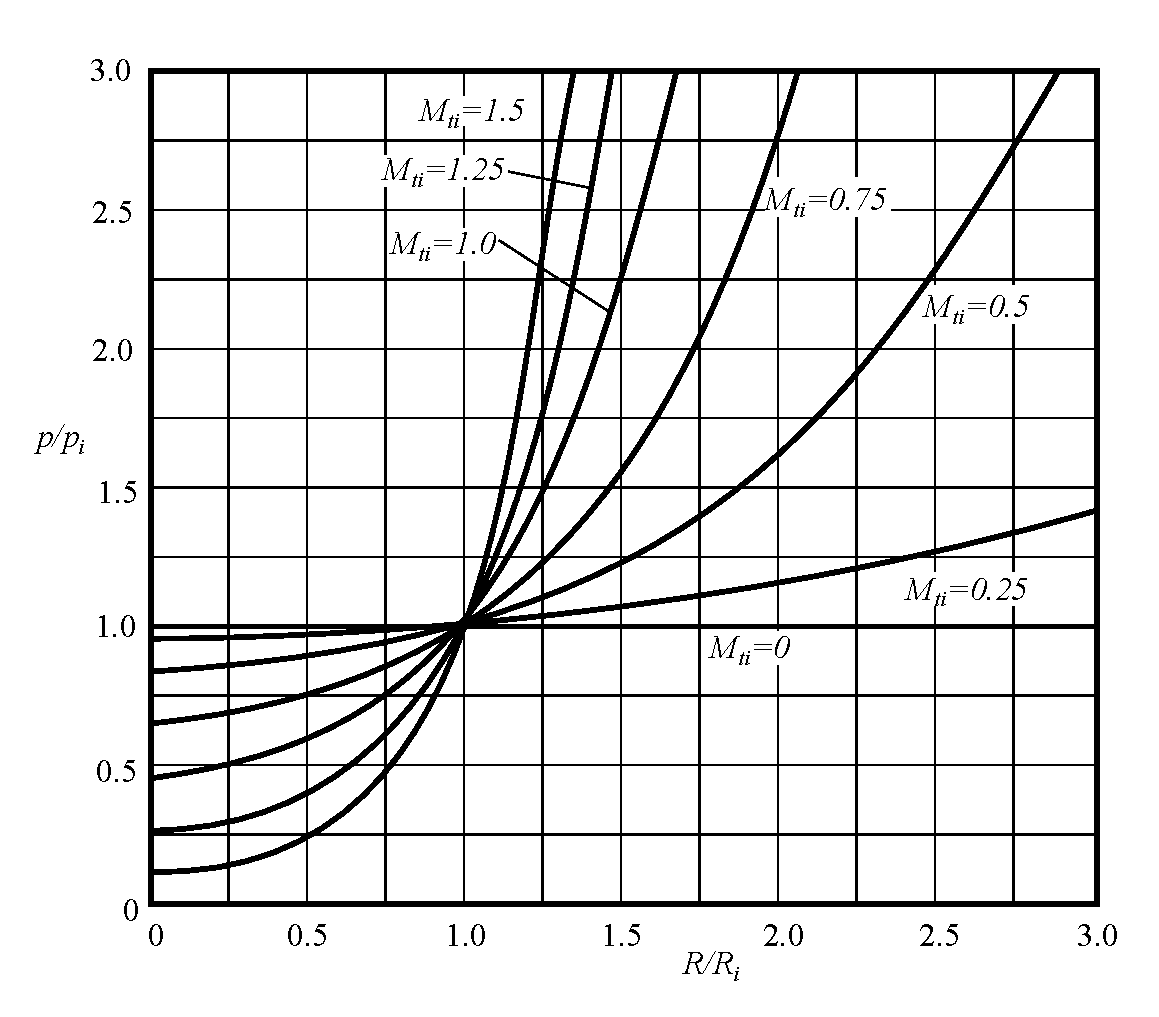
\includegraphics[width=.8\textwidth]{fig/PVortForz.pdf}
\caption{}
\label{fig:PVortForz}
\end{figure}
\\Naturalmente si può ricavare l'andamento delle pressioni e delle entalpie (Figura \ref{fig:PVortForz}); ricordando che:
\begin{align*}
\frac{p}{p_i} = \frac{h}{h_i}^{\frac{k}{k-1}}
\end{align*}
allora:
\begin{align*}
\frac{h}{h_i} = 1 + \frac{k-1}{2} M_{ti}^2 \bigg[ \bigg(\frac{r}{r_i} \bigg)^2-1 \bigg]
\end{align*}
\\L'entalpia varia con il raggio in maniera quadratica con una costante che dipende dal numero di Mach tangenziale. Si vede che con raggio pari a $0$ le pressioni non sono nulle (al contrario del caso di vortice libero). Sebbene non si realizzerà mai una macchina con vortice forzato, nel caso il diametro all'albero sia particolarmente ridotto si può utilizzare una distribuzione diversa dal vortice libero. 
\subsection{A valle del vortice forzato}
Cosa succede però a valle della palettatura dopo aver attraversato un vortice forzato? A valle è stata imposta la condizione di entalpia totale costante al variare del raggio:
\begin{align*}
\frac{dh_{01}}{dr} = 0
\end{align*}
\begin{center}
\begin{tabular}{l l l l l l l l l l l l l l l}
	Sezione 1 & & & & & & & & & & & & & & Sezione 2\\
	$
	\begin{cases}
		h_{01} = cost\\
		V_{t1} = K_1 \cdot r
	\end{cases}$ & & & & & & & & & & & & & & $V_{t2} = K_2 \cdot r$
\end{tabular}
\end{center}
Si può calcolare il lavoro scambiato come differenza di entalpia totale:
\begin{align*}
\begin{split}
h_{02} - h_{01} &= u (V_{t2} - V_{t1} ) = \omega r (K_2 r - K_1 r) \\
&= \omega (K_2 - K_1) r^2 = \Delta h_{012}
\end{split}
\end{align*}
ovvero $\Delta h \propto r^2 \; \Rightarrow \; h_{02} \neq  cost$. Quindi attraversando la macchina, a seconda del raggio ci si trova, cambia il lavoro scambiato dalla macchina; questa variazione precisa è una condizione pressoché impossibile da mantenere in fase di progettazione.\\
Si vede ora cosa succede calcolando il differenziale dell'entalpia rispetto al raggio:
\begin{align*}
\begin{split}
\cfrac{d \Delta h_{012}}{dr} &= \cfrac{d ( h_{02}-h_{01})}{dr} = \cfrac{dh_{02}}{dr} = V_a \cfrac{dV_a}{dr} + \cfrac{V_t}{r} \cfrac{d}{dr} (V_t \cdot r) = \\
& =2 \omega (K_2 - K_1) r = \cfrac{d}{dr} \bigg( \cfrac{V_{a2}^2}{2} \bigg) + K_2 \cfrac{d}{dr} (K_2 r^2)
\end{split}
\end{align*}
Anche questa è un'equazione differenziale lineare di primo ordine, che si può risolvere come:
\begin{equation}
\boxed{V_{a2}^2 = -2 \left[ K_2^2 - \omega \left( K_2 - K_1 \right) \right] r^2 + C}
\label{eq:valleVorticeForzato}
\end{equation}
La costante C si ottiene integrando su tutta la sezione la portata in massa:
\begin{align*}
\frac{\dot{m}}{2 \pi \rho} = \int_{rh}^{rs} V_{a1} r dr = \int_{rh}^{rs} V_{a2} r dr
\end{align*}
\begin{figure}[h]
\centering
  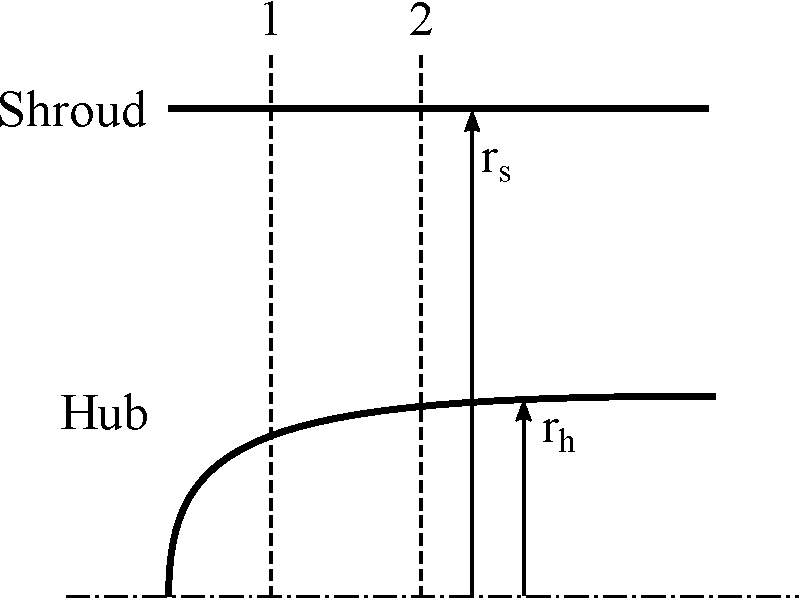
\includegraphics[width=.4\textwidth]{fig/HubShroud.pdf}
\caption{}
\label{fig:hubshroud}
\end{figure}
La portata entrante nella sezione 1 deve essere uguale alla portata che entra nella sezione 2 (integrale da resimo-hub a resimo-shroud in Figura \ref{fig:hubshroud}).
\section{Vortice generico}
Spesso nella progettazione delle macchine assiali si usa una soluzione mista tra vortice libero e forzato. Si parla di vortice generico:
\begin{align*}
\begin{cases}
V_{t1} = a \cdot r^n - \frac{b}{r}\\
V_{t2} = a \cdot r^n + \frac{b}{r}
\end{cases}
\end{align*}
Definizioni:
\begin{itemize}
\item $n=0$: zero power blending
\item $n=1$: fast power blending
\end{itemize}
Il lavoro effettuato vale quindi:
\begin{align*}
L_u = h_{02} - h_{01} = u \left( V_{t2} - V_{t1} \right) = 2 \cdot b \cdot \omega
\end{align*}
\'E da notare che il lavoro effettuato non varia con il raggio.\\
Per $n=1$ si ha una palettatura a grado di reazione costante e si può scrivere:
\begin{align*}
R = 1 - \frac{V_2^2 - V_1^2}{2 L_u} = 1 - \frac{V_{t2}^2 + \cancel{V_{a2}^2} - V_{t1}^2 - \cancel{V_{a2}^2}}{2 L_u}
\end{align*}
Considerando $V_{a2} \simeq V_{a1}$ (non è del tutto vero ma si assume la differenza piccola):
\begin{align*}
R = 1 - \frac{\cancel{\left( V_{t2} - V_{t1} \right)} \left( V_{t2}+ V_{t1} \right)}{2 u \cancel{\left( V_{t2}- V_{t1} \right)}} = 1- \frac{\left( V_{t2}+ V_{t1} \right)}{2 u} = 1-\frac{a}{\omega} = cost
\end{align*}
In questo modo si è dimostrato il grado di reazione costante nella attraversamento della macchina.
\subsection{Angolo di palettatura costante}
Si immagini ora di voler costruire una macchina con angolo di palettatura costante, ossia con il bordo di attacco rettilineo e solo la coda della palettatura cambia l'angolo.
\begin{align*}
\frac{V_t}{V_a} = \tan \alpha = cost
\end{align*}
Ci si chiede dunque come variano $V_t$ e $V_a$ al variare di $r$ rispettando l'equilibrio radiale.
Si avrà:
\begin{align*}
\frac{V}{V_i} = \frac{V_a}{V_{ai}} = \frac{V_t}{V_{ti}} = \bigg(\frac{r_i}{r} \bigg)^{\sin \alpha}
\end{align*}
Con le solite ipotesi semplificative:
\begin{align*}
\begin{cases}
\cfrac{dh_0}{dr} = 0\\
\cfrac{ds}{dr} = 0 
\end{cases}
\end{align*}
si ottiene:
\begin{align*}
\frac{d}{dr} \bigg(\frac{V_a^2}{2} \bigg) + \frac{V_t}{r} \frac{d(rV_t)}{dr} = 0
\end{align*}
Sapendo inoltre che:
\begin{align*}
\begin{cases}
V_a = V \cos \alpha\\
V_t = V \sin \alpha
\end{cases}
\end{align*}
e facendo le opportune sostituzioni si perviene a:
\begin{align*}
\frac{dV}{dr} + \frac{V}{r} \sin^2 \alpha = 0
\end{align*}
L'equazione differenziale è leggermente più complessa; la soluzione generica è di tipo esponenziale e bisogna sempre andare a determinare la costante generica.
\begin{align*}
y' + \varphi(x)y + \psi(x) = 0 
\end{align*}
\begin{align*}
y = e^{-\int \varphi(x)dx} \bigg[ C- \int \psi(x) e^{\int \varphi(x)dx} dx \bigg] 
\end{align*}
Nel caso in analisi $\psi(x) = 0$ quindi:
\begin{align*}
V = e^{-\int \frac{\sin^2 \alpha}{r}dr}\cdot C = r^{-\sin^2 \alpha} \cdot C
\end{align*}
Per $r=r_i,\; V=V_i$ allora:
\begin{align*}
C = \frac{V_i}{r_i^{-\sin^2 \alpha}}
\end{align*}
Questo porta ad un'espressione del rapporto tra le entalpie pari a:
\begin{align*}
\boxed{ \frac{h}{h_i} =  1+ \frac{V_{ti}^2}{2 h_i \sin^2 \alpha} \bigg[1- \bigg(\frac{r_i}{r} \bigg) ^{2 \sin^2 \alpha} \bigg]}
\end{align*}
Si tratta di una soluzione adottata per le macchine a vapore che possiedono delle palettature molto massicce, con sviluppo radiale limitato che permettono di ottenere un andamento delle velocità assiali come in Figura \ref{fig:AngPalCost}. Questa è una distribuzione che non ha limiti teorici, si può sempre fare una macchina a bordo d'ingresso rettilineo; essa rappresenta un caso intermedio tra un vortice libero e un vortice forzato.\\
\'E possibile osservare nelle figura \ref{fig:TurboFan1} come cambia la svergolamento della palettatura tra Hub e Shroud di una turbina e di un compressore in caso di corrente a vortice libero; questa forma particolare ha il fine di mantenere le condizioni di equilibrio radiale visto che cambia il profilo di velocità della corrente.
\begin{figure}
\centering
  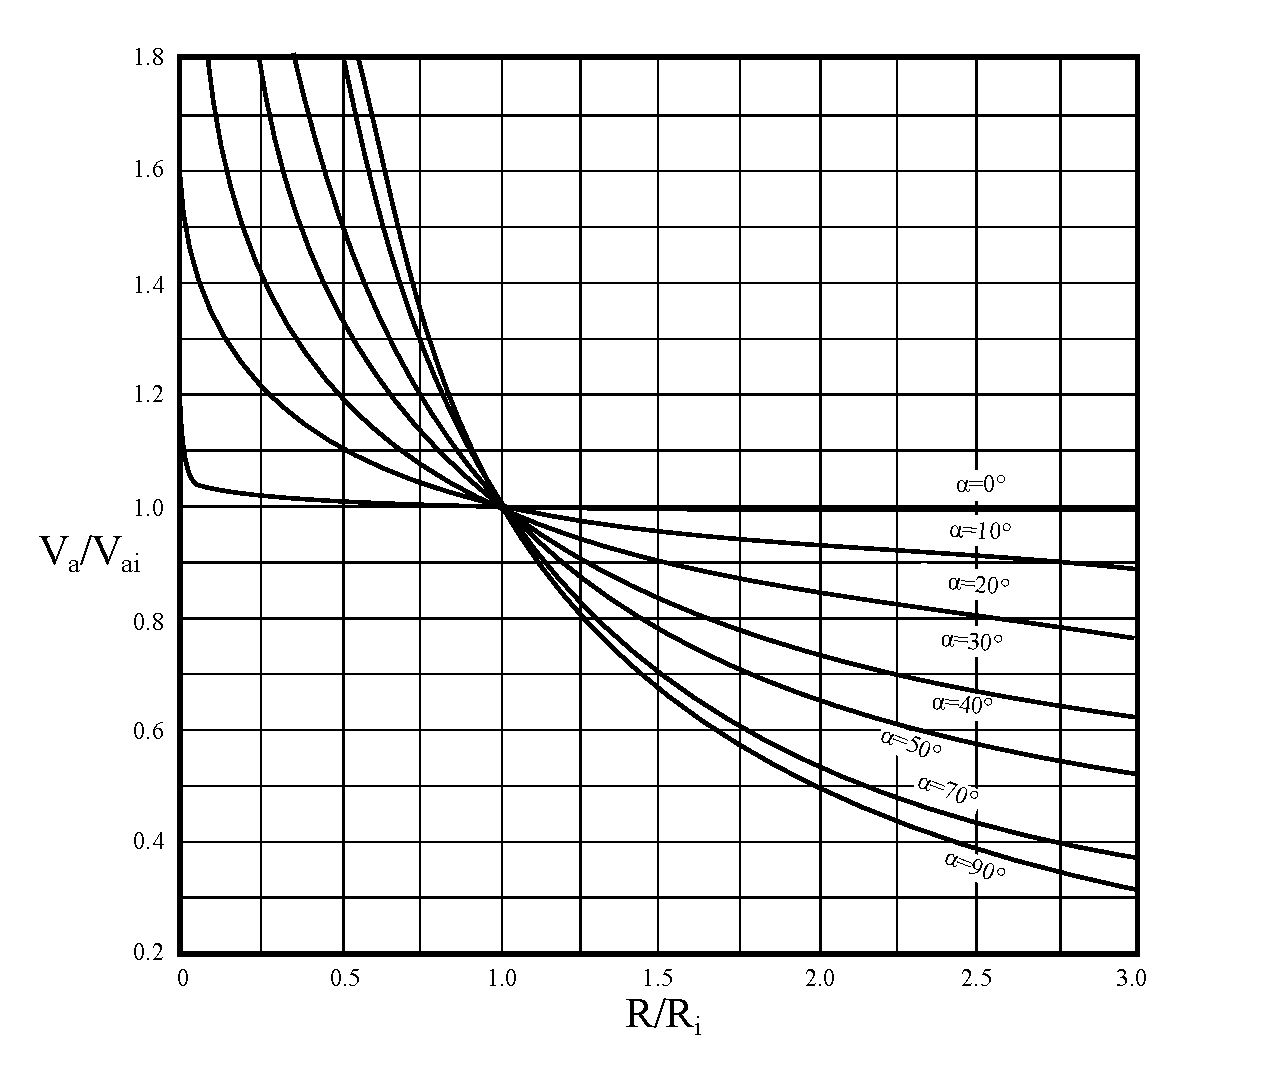
\includegraphics[width=.8\textwidth]{fig/AngPalCost.pdf}
\caption{}
\label{fig:AngPalCost}
\end{figure}
\begin{figure}
\centering
  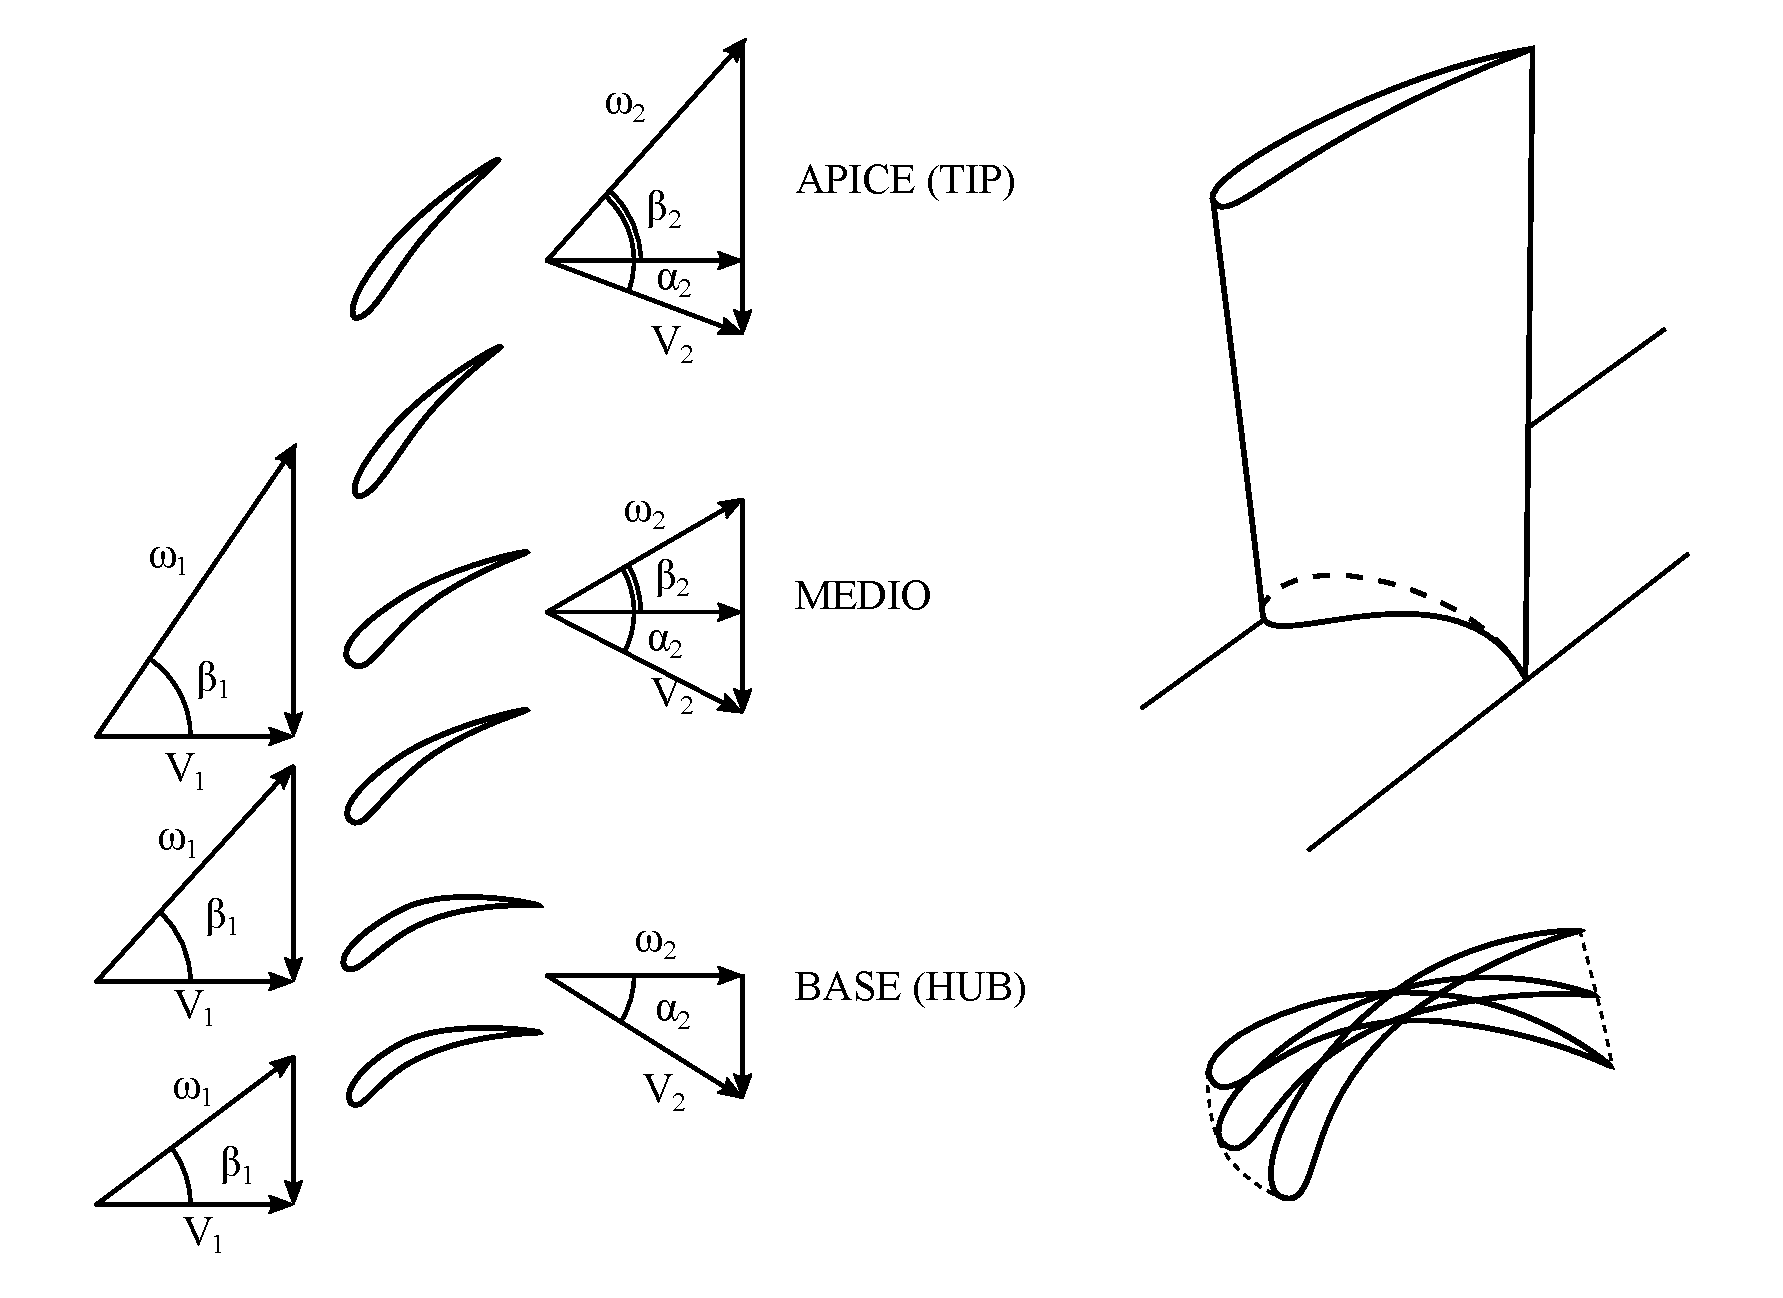
\includegraphics[width=.8\textwidth]{fig/TurboFan.pdf}
\caption{Profili e triangoli delle velocità per un rotore di turbo fan a vortice libero ($r_{Tip}/r_{Hub} =2$)}
\label{fig:TurboFan1}
\end{figure}
\begin{figure}
\centering
  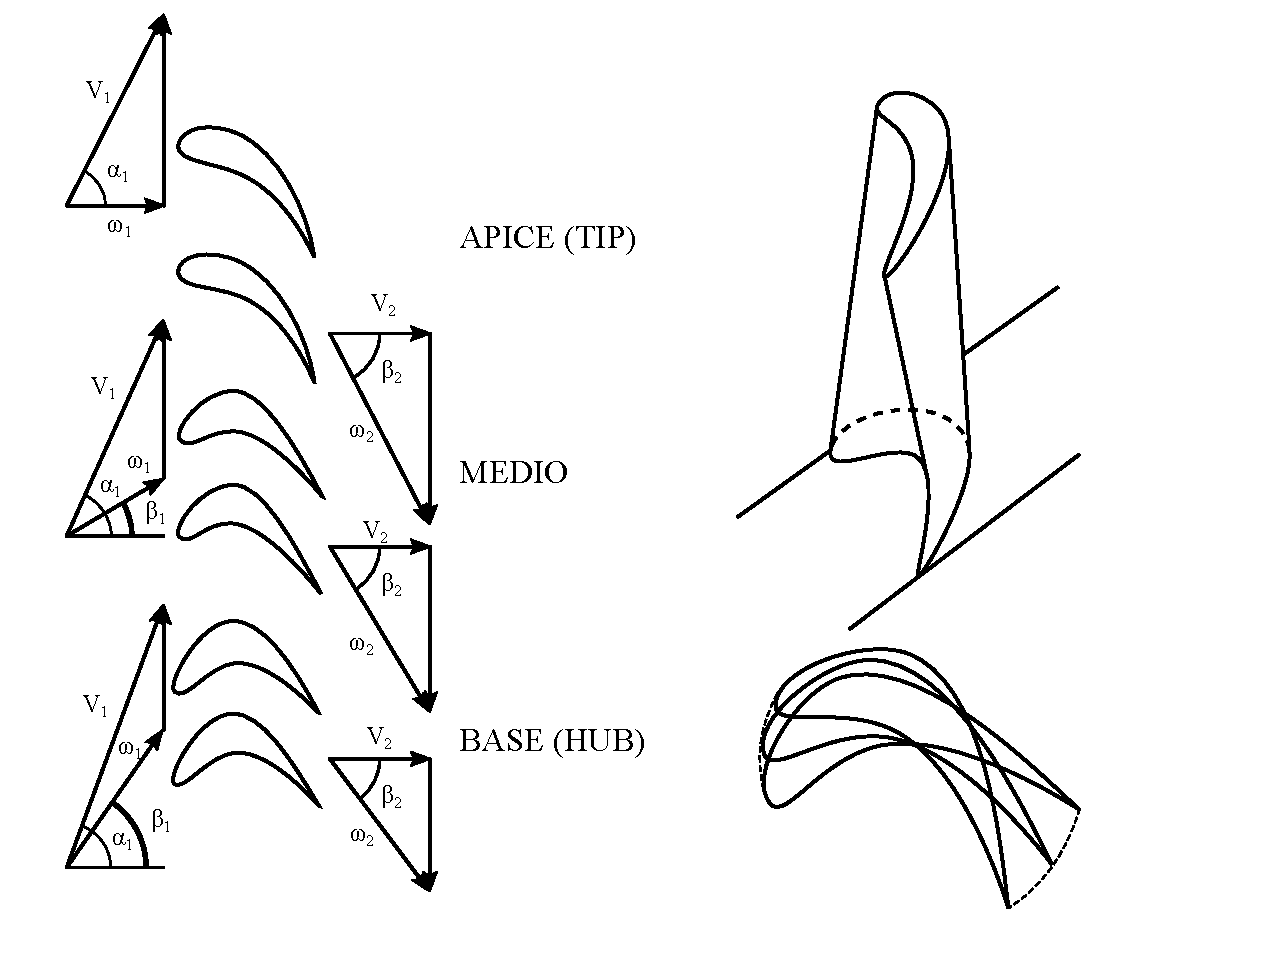
\includegraphics[width=.8\textwidth]{fig/TurbVortLib.pdf}
\caption{Profili e triangoli delle velocità per un rotore di uno stadio di bassa pressione di turbina a vapore o a gas ($r_{Tip}/r_{Hub} =1.4$)}
\label{fig:TurbVortLib}
\end{figure}
\section{Portata in un condotto anulare}
Si analizzano ora quali sono le altre particolarità del flusso nell'attraversamento della macchina, in particolare quello che accade in un condotto anulare. Si definisce la portata generica tra l'hub e lo shroud integrando tra questi due estremi:
\begin{align*}
\dot{m} = 2 \pi \int_{rh}^{rs} \rho V_a r dr
\end{align*}
con $V_a$ dipendente dal vortice utilizzato per progettare l'andamento dei triangoli di velocità ai diversi raggi. Questa espressione è limitata al caso di flusso comprimibile.\\
Considerando una sezione anulare piccola, quindi $V_a = cost$, si scrive:
\begin{align*}
\dot{m} = S \rho V_a = S \rho_0 a_0 \Phi = cost \cdot \Phi
\end{align*}
\begin{equation}\label{eq:portanulare}
\Phi = \frac{\rho}{\rho_0} \frac{V_a}{a_0}
\end{equation}
Si valutano ora i rapporti che compaiono nell'equazione \ref{eq:portanulare}, la quale rappresenta la portata adimensionalizzata rispetto le condizioni di ristagno a monte sotto l'ipotesi di gas perfetto $p = \rho RT$ e flusso isoentropico $p \rho^{-k} = cost$.\\
Si scrive scrivere il rapporto $\rho/\rho_0$ nel seguente modo:
\begin{align*}
\frac{\rho}{\rho_0} = \bigg( \frac{T}{T_0} \bigg)^{\frac{1}{k-1}} 
\end{align*}
ma scrivendo:
\begin{align*}
\begin{cases}
a = \sqrt{kRT}\\
a_0 = \sqrt{kRT_0}
\end{cases}
\end{align*}
\begin{align*}
\frac{\rho}{\rho_0} = \bigg( \frac{a}{a_0} \bigg)^{\frac{2}{k-1}}
\end{align*}
Si sviluppa ora il secondo rapporto:
\begin{align*}
V^2 = 2 (h_0 - h) = 2 c_p (T_0 - T) = 2 \frac{c_p}{kR} (a_0^2 - a^2)
\end{align*}
\begin{align*}
\frac{V_a^2}{a_0^2} = \frac{2}{k-1} \bigg[ 1- \bigg( \frac{a}{a_0} \bigg)^2 \bigg] = \frac{V_a^2 + V_t^2}{a_0^2}
\end{align*}
\begin{align*}
\frac{V_a}{a_0} = \sqrt{\frac{2}{k-1} \bigg[ 1- \bigg( \frac{a}{a_0} \bigg)^2 \bigg] - \bigg( \frac{V_t}{a_0} \bigg)^2}
\end{align*}
Sostituendo nell'espressione della portata risulta:
\begin{align*}
\Phi = \frac{\rho}{\rho_0} \frac{V_a}{a_0} = f \bigg( \frac{a}{a_0} \bigg)
\end{align*}
Si cerca ora il rapporto critico tra le velocità soniche che massimizzano la portata. Se la componente di velocità tangenziale fosse nulla e quindi moto monodimensionale, l'espressione sarebbe quella della velocità critica di un condotto convergente in cui si arriva alla condizione di choking
\begin{align*}
\frac{d\Phi}{d \bigg( \frac{a}{a_0} \bigg)} \; \Rightarrow \; \boxed{ \frac{a^*}{a_0} = \sqrt{\frac{2}{k+1} - \frac{k-1}{k+1} \bigg( \frac{V_t}{a_0} \bigg)^2} }
\end{align*}
con
\begin{align*}
Ma^* = \bigg( \frac{V_a}{a} \bigg)^* = 1
\end{align*}
Diagrammando l'andamento di $\Phi$ in funzione del rapporto di $p/p_0$, risulta una portata adimensionale di un flusso elicoidale in funzione della pressione e delle diverse componenti tangenziali (figura \ref{fd:PortCondAn}).\\
Il flusso in un condotto anulare, può essere supersonico ma non in condizioni di choking, a patto che la velocità assiale sia inferiore a quella acustica. Il choking si ha in tre casi:
\begin{itemize}
\item raggiungimento di velocità sonica $V$ nello statore;
\item raggiungimento di velocità sonica $W$ nel rotore;
\item raggiungimento di velocità sonica assiale nel condotto anulare.
\end{itemize}
\begin{figure}
\centering
  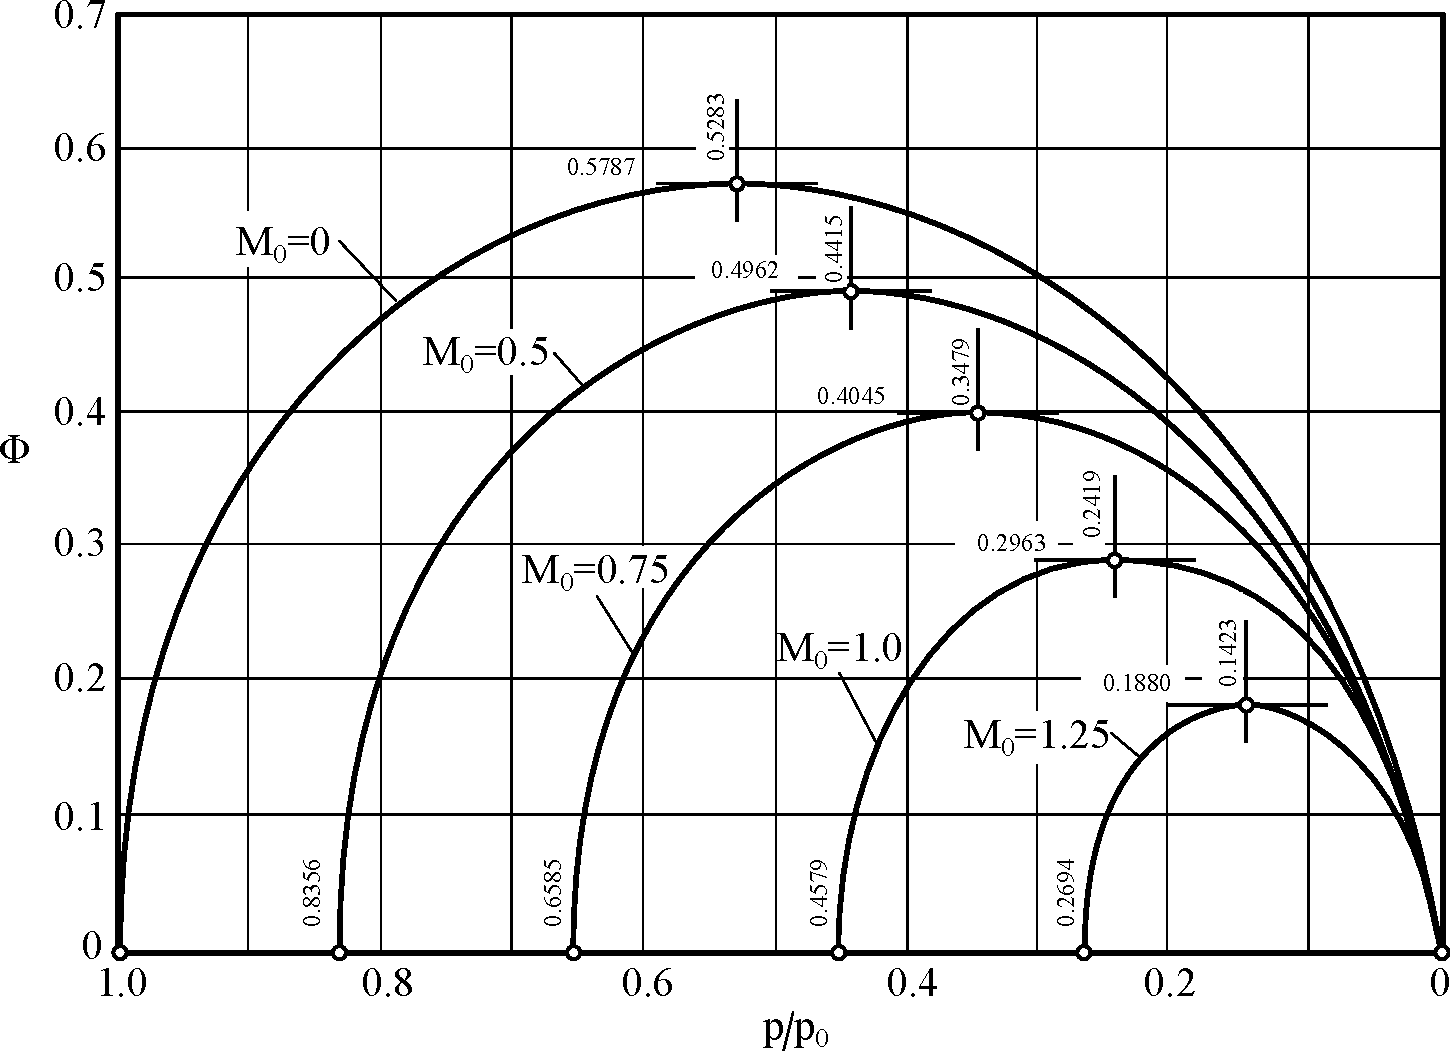
\includegraphics[width=.7\textwidth]{fig/PortCondAn.pdf}
\caption{}
\label{fd:PortCondAn}
\end{figure}
\section{Condizioni di ingolfamento (choking)}
Diminuendo la pressione a valle si aumenta la componente assiale della velocità $V_a$ pur mantenendo $V_t$, se il moto è libero, mentre non è possibile in un moto guidato dalla palettatura. Il segnale di pressione deve riuscire a propagarsi a monte e questo accade solamente se le velocità sono subsoniche.\\
Si considera un punto $P$ da cui si propaga un'onda di pressione all'interno del cono di Mach come mostrato in figura \ref{fd:bloccson1}.
\begin{itemize}
	\item Nel caso di velocità $V_a$ supersonica, la perturbazione di pressione non si propaga a monte del fronte.
	\item Nel caso di velocità $V_a$ subsonica, la perturbazione di pressione si propaga a monte del fronte; in questo modo ad una diminuzione di pressione corrisponde un aumento di velocità a monte (figura \ref{fd:bloccson2} sinistra).
	\item Nel caso ci si trovi in condizioni limite con $M_a=1$, la propagazione del segnale di pressione raggiunge esattamente il punto ``di partenza $P$" della particella come mostrato in figura \ref{fd:bloccson2} a destra; in questo caso non è quindi possibile trasmettere un segnale di pressione a monte e da questo punto in poi il flusso è ingolfato.
\end{itemize} 
\begin{figure}
\centering
  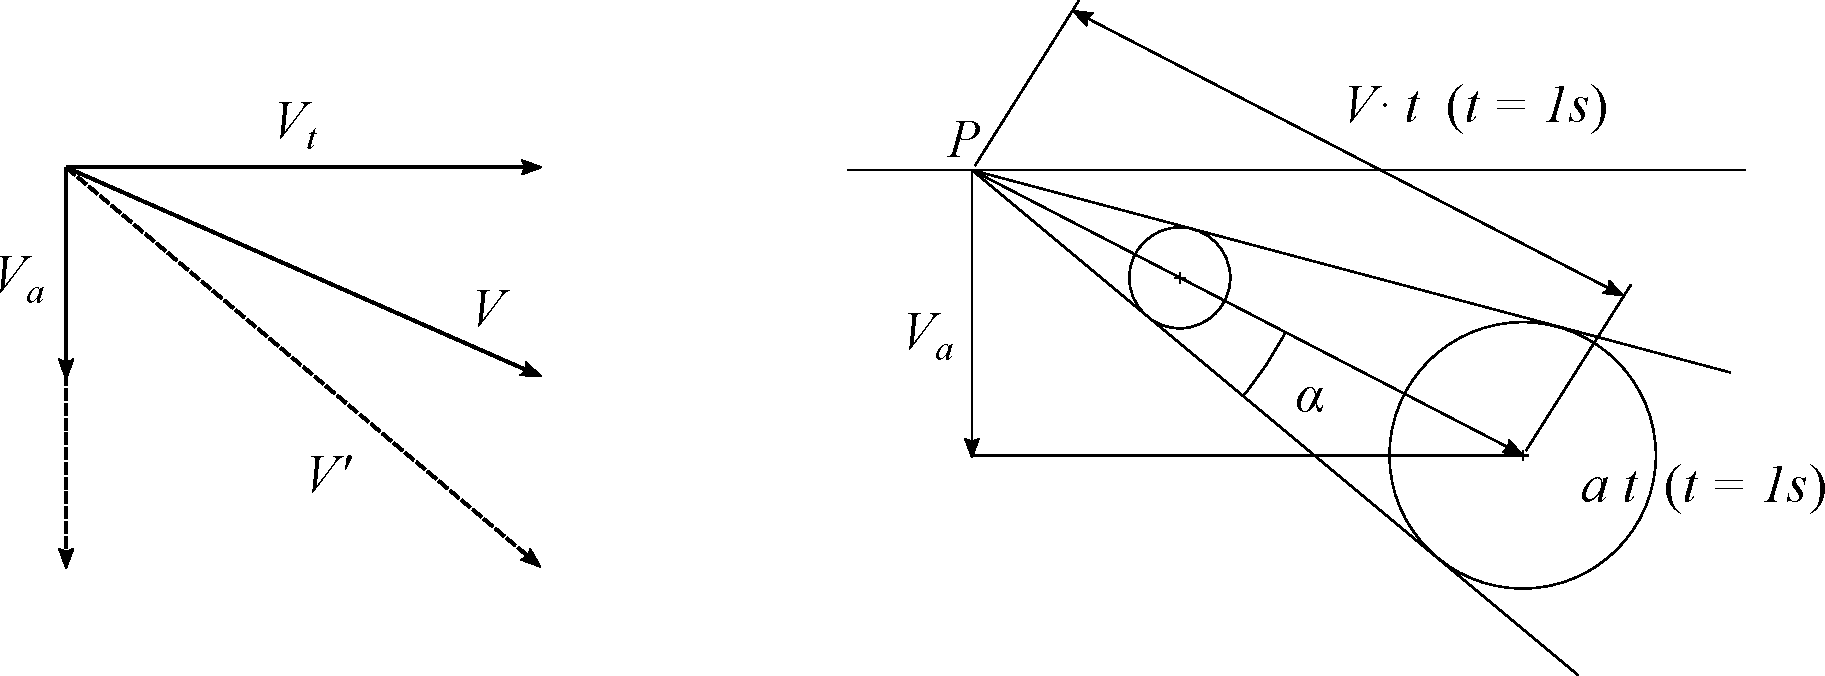
\includegraphics[width=.8\textwidth]{fig/bloccson1.pdf}
\caption{}
\label{fd:bloccson1}
\end{figure}
\begin{figure}
\centering
  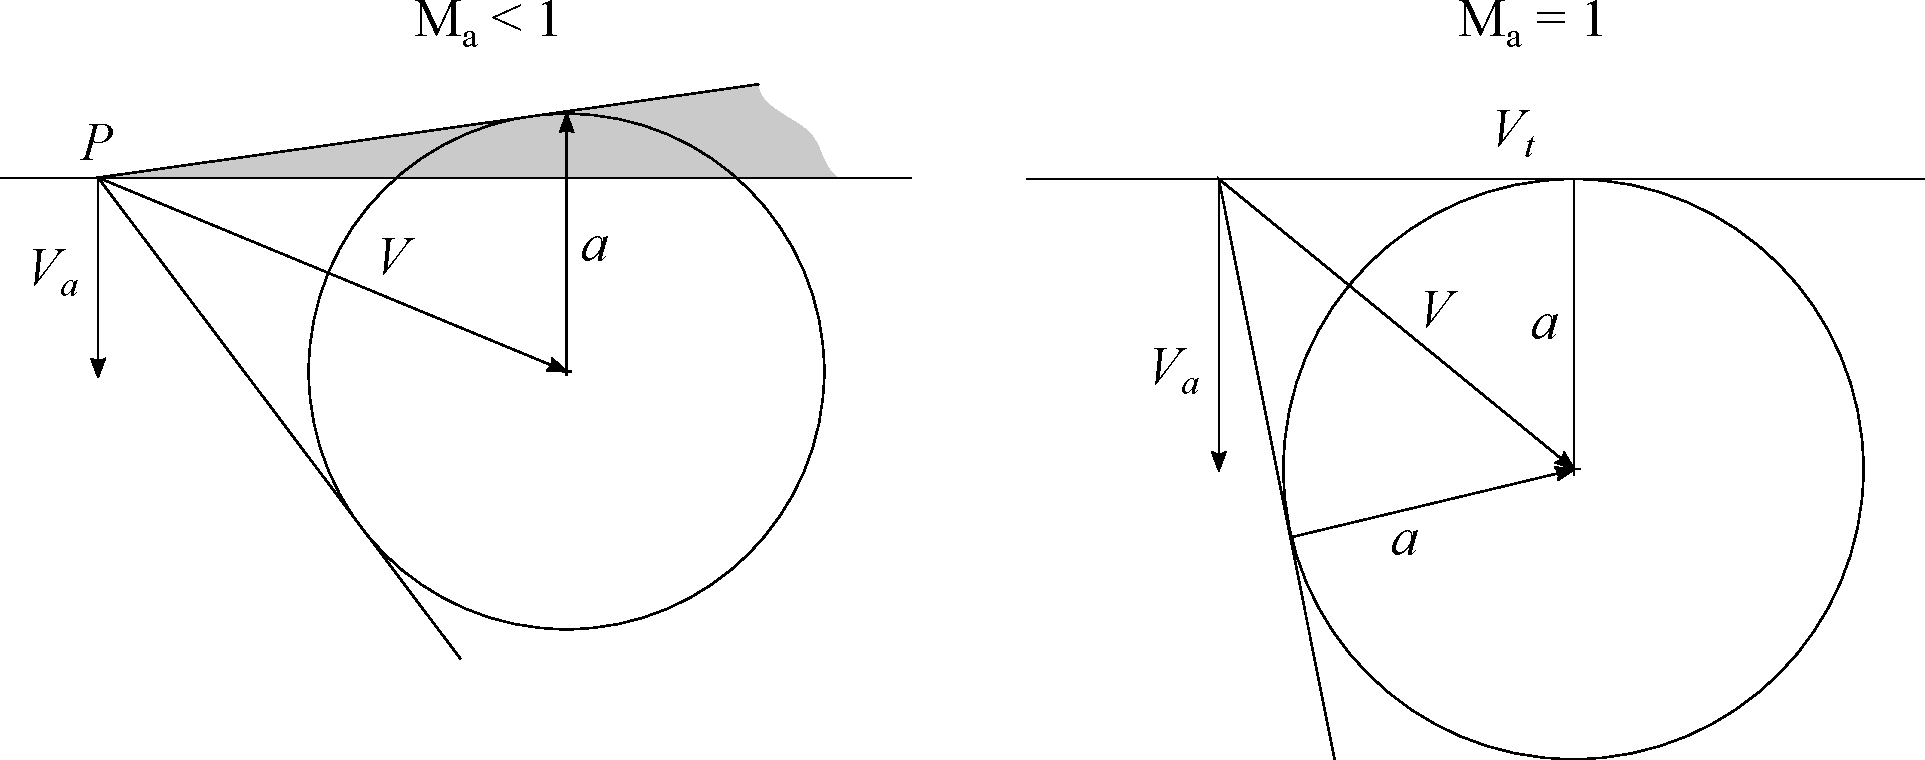
\includegraphics[width=.8\textwidth]{fig/bloccson2.pdf}
\caption{}
\label{fd:bloccson2}
\end{figure}
\section{Componente radiale non trascurabile}
Nel caso ci sia nel flusso una componente radiale non trascurabile, come nel caso mostrato in figura \ref{fd:comp_rad}, in prossimità del mozzo le equazioni dell'equilibrio radiale imposte sull'elementino di fluido evidenziato si modificano con l'aggiunta di un termine:
\begin{align*}
\frac{d h_0}{dr} - T\frac{ds}{dr} = V_a \frac{dV_a}{dr} - \boxed{V_a \frac{dV_r}{dz}} + \frac{V_t}{r} \frac{d}{dr} ( V_t \cdot r)
\end{align*}
\begin{figure}
\centering
  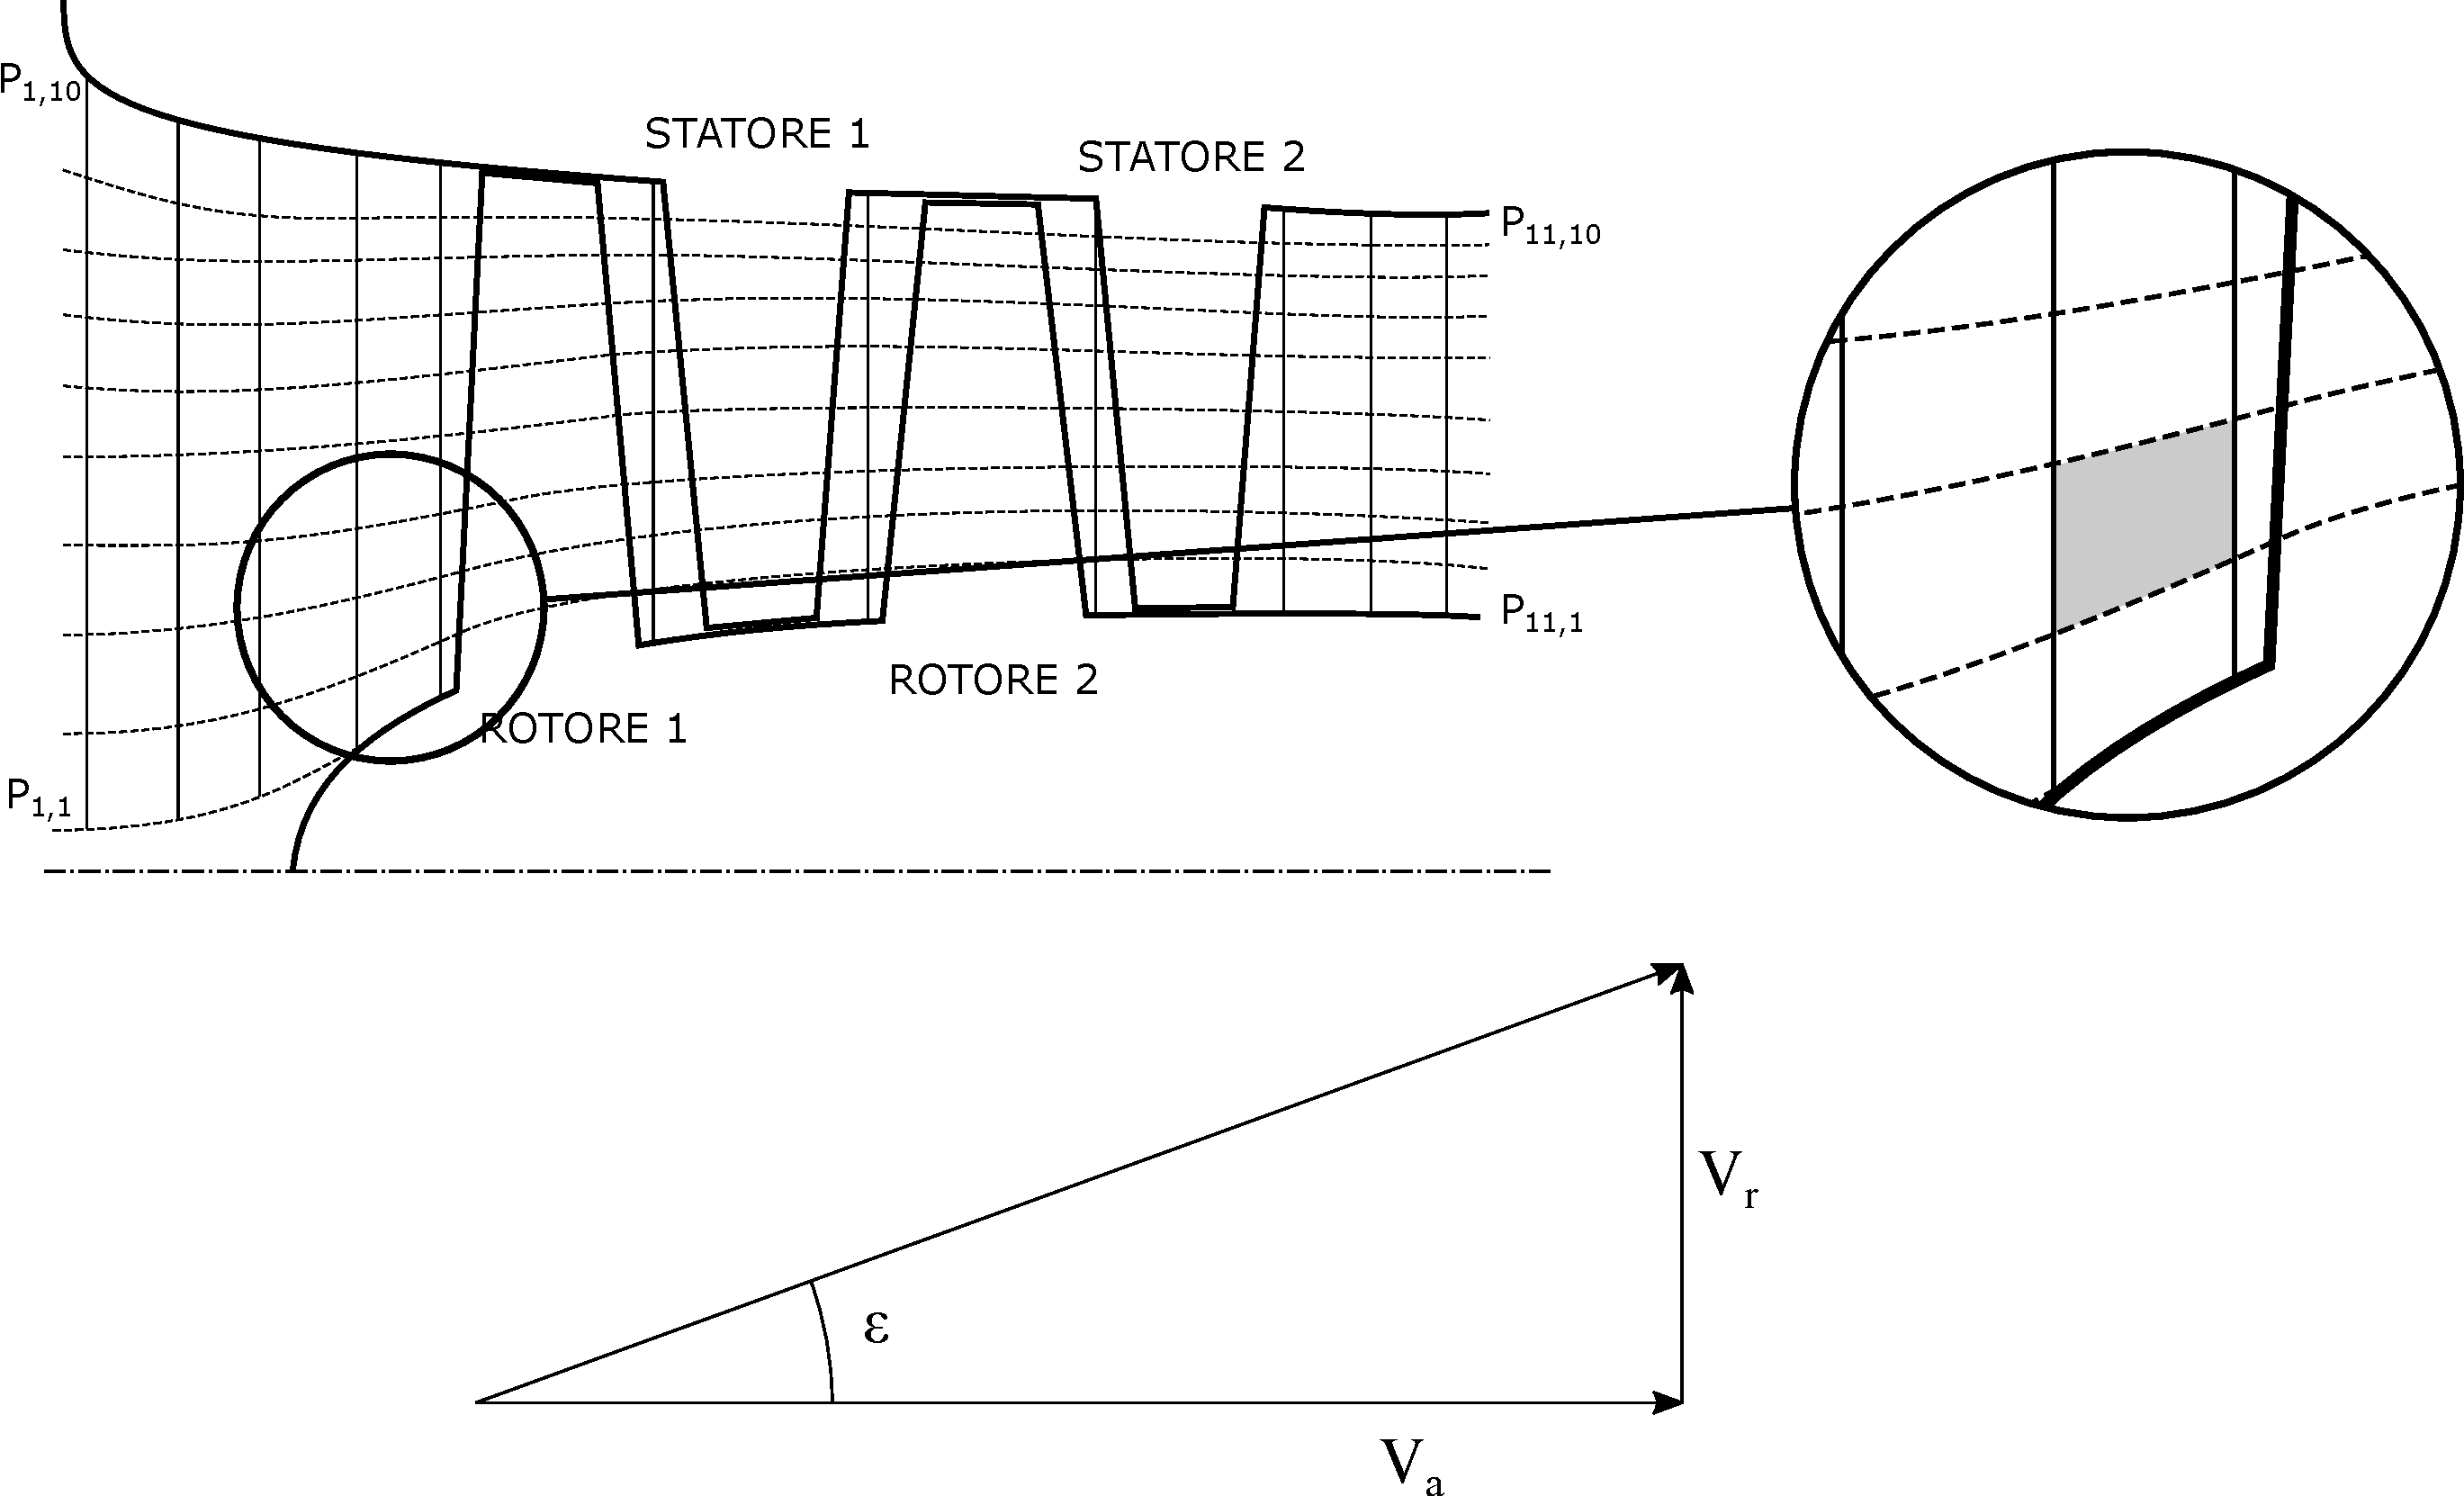
\includegraphics[width=.8\textwidth]{fig/comp_rad.pdf}
\caption{}
\label{fd:comp_rad}
\end{figure}
\section{Moti secondari}
Fino ad ora si è sempre ragionato su un flusso idealizzato che però non corrisponde alla realtà. Nella zona superiore, in cui le pale del rotore sono molto vicine alla cassa e vicino alla radice delle pale, si forma lo strato limite a parete che innesca i moti secondari a causa appunto dell'interazione del fluido con la parete. Anche se questi moti nascono in zone limitate possono comunque influenzare grosse sezioni. Ci sono quattro diverse tipologie di moti secondari:
\begin{itemize}
\item Vortici di passaggio: sono dovuti ad un moto curvato e una perturbazione dovuta allo strato limite che generano vortici con direzioni opposte (figura \ref{fig:VortPass}). Essi sono dovuti ai diversi gradienti di pressione.
\item Vortici a ferro di cavallo: sono dovuti all'interazione tra strato limite in ingresso e un ostacolo, come per esempio la palettatura (figura \ref{fd:VortFerrCav}).
\item Vortici al bordo di uscita: sono dovuti alla scia di vorticità per lo strato limite al bordo di uscita della schiera (figura \ref{fd:VortVall}).
\item Vortici di passaggio e di trafilamento: sono dovuti ai giochi tra statore e cassa (figura \ref{fd:VortTraf}).
\end{itemize}
\begin{figure}[h!]
\centering
  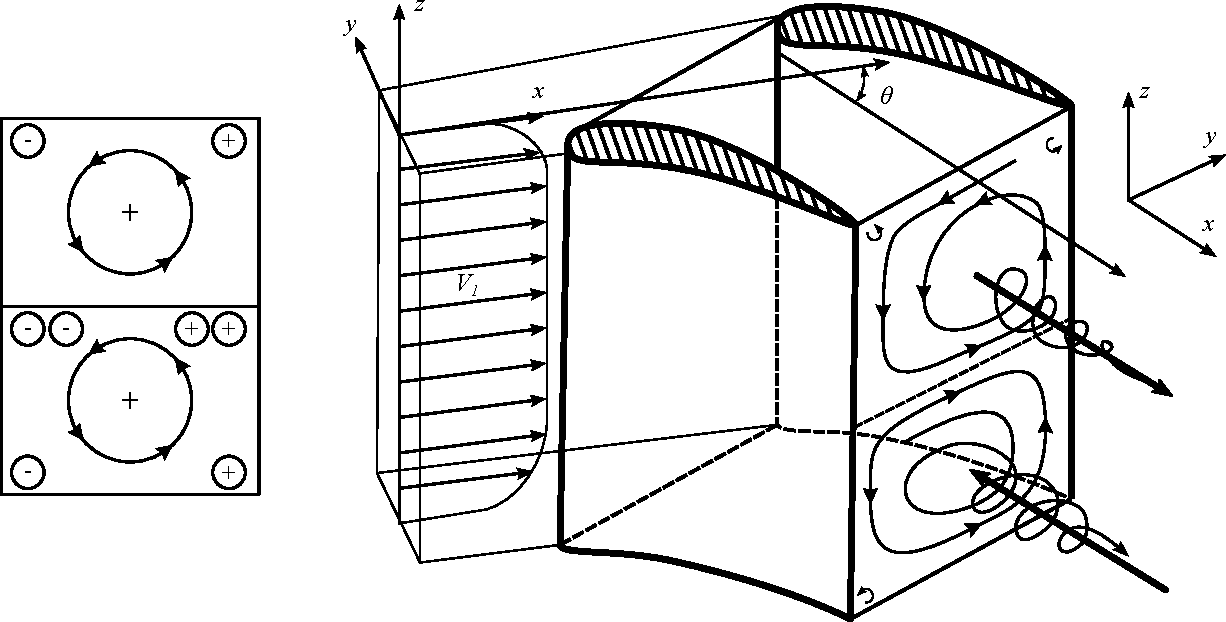
\includegraphics[width=.7\textwidth]{fig/VortPass.pdf}
\caption{}
\label{fig:VortPass}
\end{figure}
\begin{figure}[h!]
\centering
  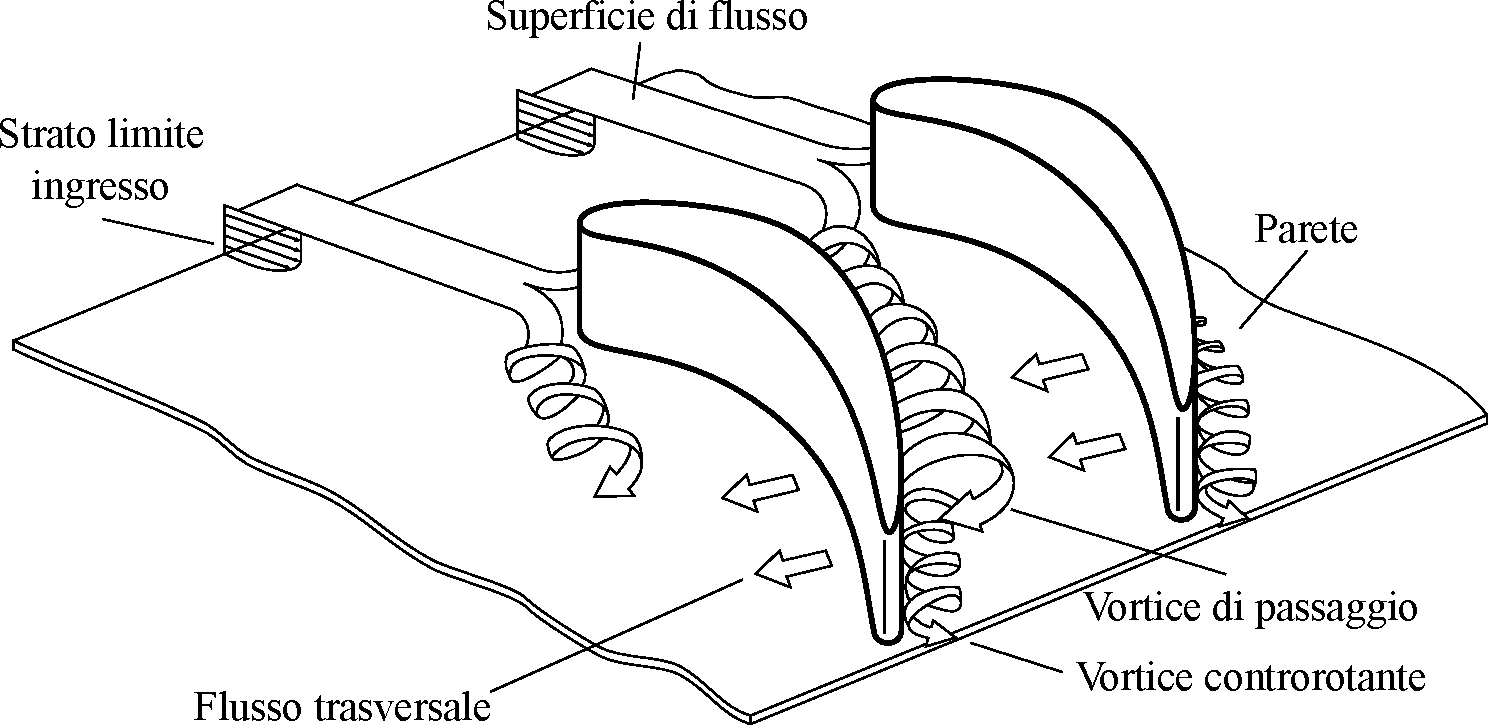
\includegraphics[width=.7\textwidth]{fig/VortFerrCav.pdf}
\caption{}
\label{fd:VortFerrCav}
\end{figure}
\begin{figure}[h!]
\centering
  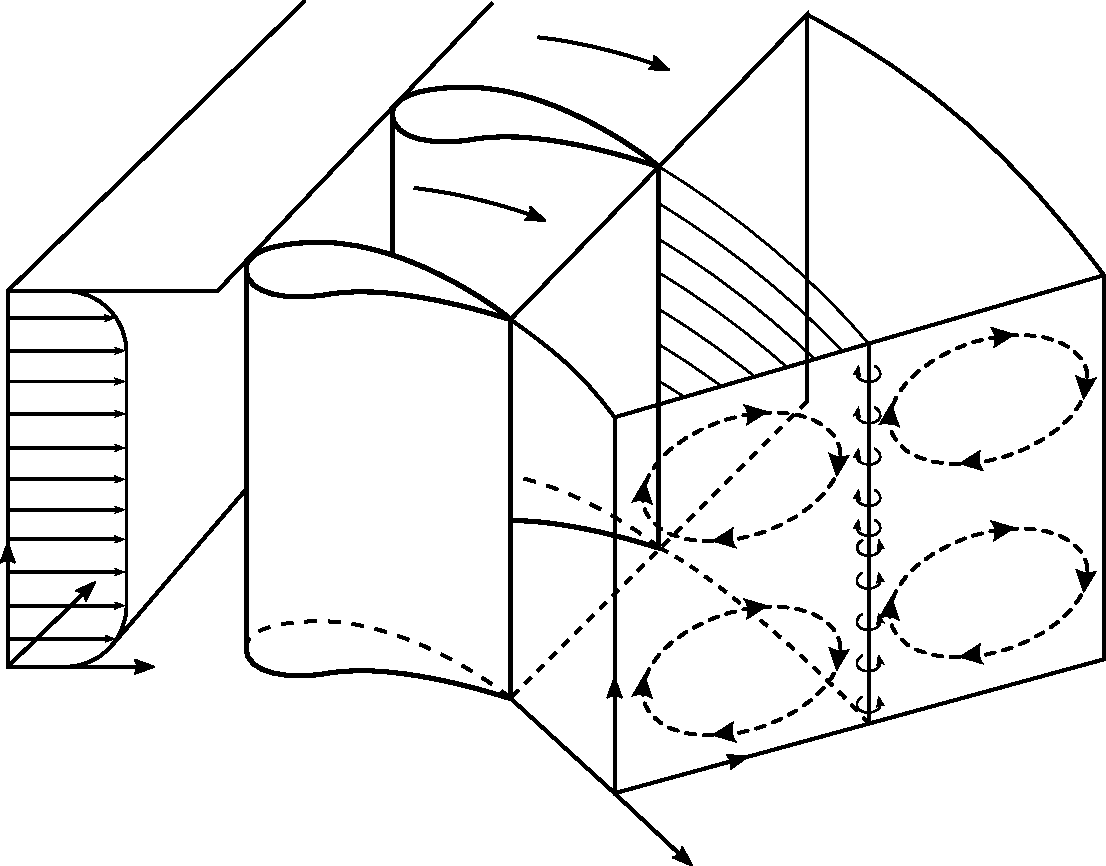
\includegraphics[width=.6\textwidth]{fig/VortVall.pdf}
\caption{}
\label{fd:VortVall}
\end{figure}
\begin{figure}[h!]
\centering
  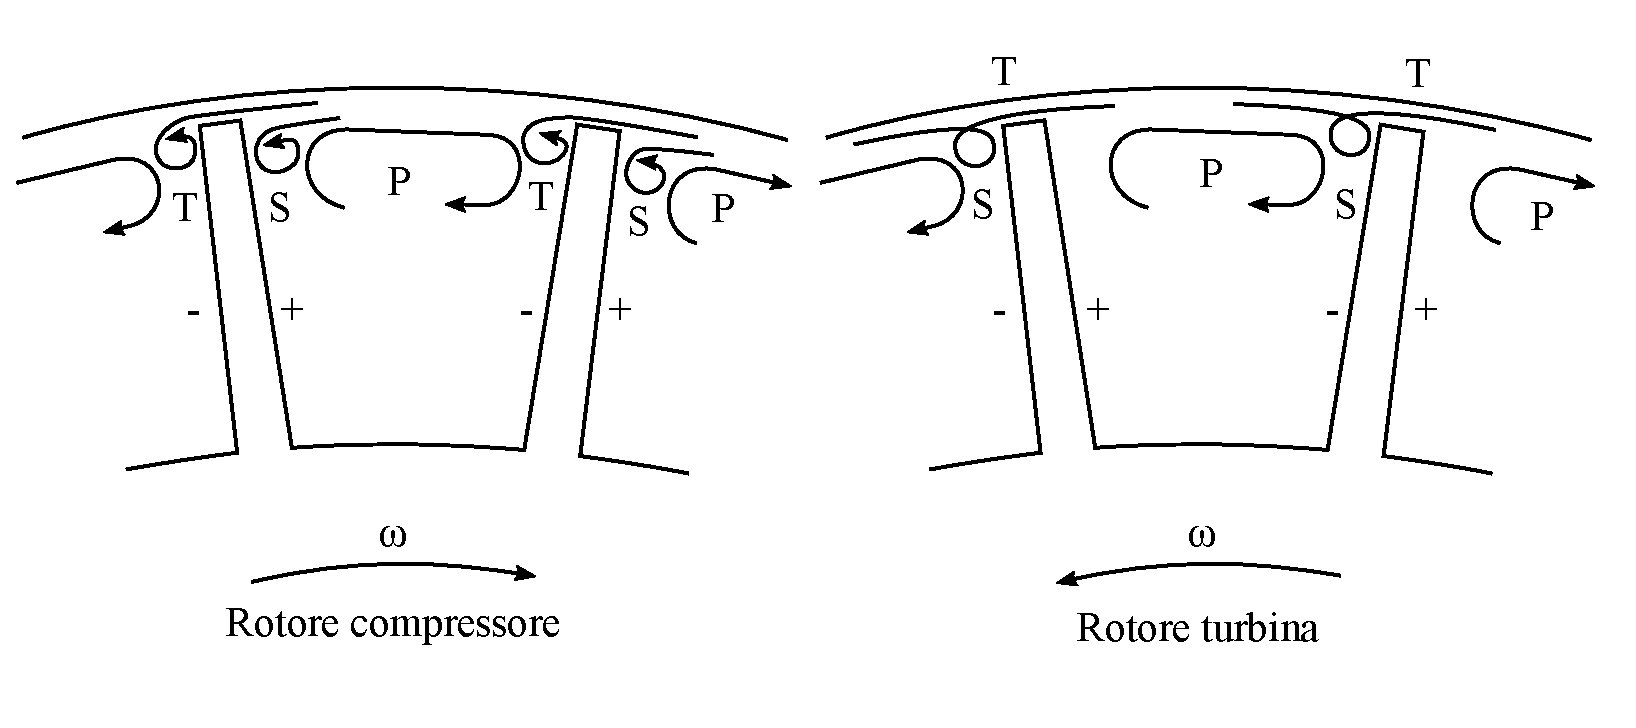
\includegraphics[width=.8\textwidth]{fig/VortTraf.pdf}
\caption{}
\label{fd:VortTraf}
\end{figure}